\documentclass{article}

\PassOptionsToPackage{numbers,sort&compress}{natbib}
\usepackage[main]{neurips_2026}
\usepackage[utf8]{inputenc}
\usepackage[T1]{fontenc}
\usepackage{hyperref}
\usepackage{url}
\usepackage{booktabs}
\usepackage{amsmath}
\usepackage{amssymb}
\usepackage{microtype}
\usepackage{xcolor}
\usepackage{graphicx}
\usepackage{subcaption}
\usepackage{enumitem}

\definecolor{phlox}{HTML}{CAA9F3}
\definecolor{verbena}{HTML}{B37AD4}
\definecolor{periwinkle}{HTML}{7997E6}
\definecolor{atlantis}{HTML}{206ABC}
\definecolor{phthaloblue}{HTML}{0E155E}
\hypersetup{colorlinks=true,linkcolor=phthaloblue,citecolor=atlantis,urlcolor=atlantis}

\title{Language-Model Control of Adaptive Batch Active Learning for Ligand Discovery}

\author{Anonymous Authors}

\begin{document}

\maketitle

\begin{abstract}
Batch active learning for ligand discovery requires a recurring decision about whether to exploit high predicted affinity, reduce model uncertainty, or broaden chemical coverage. We test whether a language model can make this strategy-level decision from leakage-safe summaries while a deterministic Gaussian-process environment retains control of candidate ranking and label revelation. Across four protein targets, ten paired seeds, and a 360-compound assay budget, a GPT-5.6 Sol controller outperformed random sampling in all 40 matched campaigns. Its final top-2\% recall was 0.412 on D2R, 0.374 on Mpro, 0.448 on TYK2, and 0.683 on USP7. It was statistically tied with the strongest fixed policy on Mpro and USP7 but underperformed target-specific leaders on D2R and TYK2. The controller shifted from exploration-oriented early batches toward exploitation and produced 686 testable threshold claims with an 86.3\% atomic success rate, although 19.8\% of forecasts were not numerically scorable. In 200 prespecified information-ablation campaigns, removing uncertainty, diversity, or memory caused only small endpoint changes, while shuffling explanatory evidence reproduced the full allocation path in 39 of 40 paired campaigns. A deterministic 80\% availability constraint reduced recall on every target but preserved the target-dependent pattern of wins and losses. These results support language-model strategy control as a feasible and auditable layer, while showing that universal superiority and causal use of explanations remain unestablished.
\end{abstract}

\section{Introduction}

Experimental ligand discovery is a search problem under a strict measurement budget. Active learning uses observations collected so far to choose the next compounds, ideally concentrating assays on high-value regions without losing the information needed to improve the model. Early work demonstrated that active selection can outperform random screening in drug discovery \citep{warmuth2001active}, while later work showed that batch selection introduces a cost of parallelization and makes diversity important \citep{jiang2018batch}. Gaussian-process (GP) surrogates are attractive because they provide both predictions and uncertainty, enabling acquisition rules that trade off exploitation and information gathering \citep{srinivas2010gpucb}.

No single acquisition strategy is expected to dominate every chemical landscape. The four-target benchmark that supplies our data and software found substantial dependence on the target, representation, kernel, and acquisition policy \citep{srivastava2026explainable}. This suggests a meta-control problem: instead of freezing one acquisition mixture for an entire campaign, can a controller alter the mixture after observing campaign progress?

We evaluate a constrained language-model controller that never sees hidden affinities and never directly selects unrestricted molecules. At each cycle it allocates a batch among three deterministic queues: high predicted mean, high posterior uncertainty, and chemical diversity. The design separates language-model judgment from numerical modeling and assay simulation. Our contributions are:

\begin{itemize}[leftmargin=*,nosep]
    \item a paired four-target benchmark comparing 40 agent campaigns with 360 fixed-policy campaigns;
    \item an auditable protocol that records every allocation, rationale, expected outcome, selected index, and revealed result;
    \item outcome scoring for testable rationale claims and 200 prespecified information-ablation campaigns; and
    \item an operational extension in which only a deterministic 80\% of post-initial candidates are available.
\end{itemize}

\section{Related work}

Active search prioritizes finding members of a valuable class rather than only minimizing predictive error. Drug discovery was an early motivating application \citep{warmuth2001active}. Nonmyopic batch active search formalized the simultaneous selection setting and demonstrated the importance of diversity in batch construction \citep{jiang2018batch}. Bayesian optimization and GP upper-confidence methods provide a complementary view in which posterior mean and uncertainty guide expensive evaluations \citep{srinivas2010gpucb}.

Molecular fingerprints encode local structural environments in fixed-length vectors; extended-connectivity fingerprints remain a widely used representation \citep{rogers2010ecfp}. Similarity kernels, including Tanimoto-style kernels, allow kernel machines and GPs to operate on fingerprint representations \citep{ralaivola2005kernels}. Our experiments extend the explainable active-learning framework and four target datasets of \citet{srivastava2026explainable}. The new element is a language model acting only as the allocation controller, not as the molecular predictor or assay oracle.

\section{Methods}

\subsection{Datasets and representation}

We use four ligand-affinity datasets: D2R (2,502 compounds), Mpro (2,749), TYK2 (9,997), and USP7 (1,799). Each table contains unique, nonempty SMILES and a finite affinity value. Molecules are represented by 4,096-bit Morgan fingerprints with radius 4, consistent with extended-connectivity representations \citep{rogers2010ecfp}. A small exact GP uses a fixed Tanimoto kernel, observation noise 0.05, and numerical jitter $10^{-6}$.

\subsection{Campaign protocol}

Each campaign begins with 60 randomly measured compounds. Ten cycles add 30 compounds each, producing a final budget of 360. For every target and seed, all methods share the same initial set. After fitting the GP to revealed labels, the environment constructs three ordered queues from the remaining pool:

\begin{align}
Q_{\mathrm{exploit}} &: \text{descending posterior mean}, \\
Q_{\mathrm{uncertain}} &: \text{descending posterior standard deviation}, \\
Q_{\mathrm{diverse}} &: \text{descending novelty relative to measured compounds}.
\end{align}

The controller emits nonnegative integers $(n_e,n_u,n_d)$ satisfying $n_e+n_u+n_d=30$. The environment then selects unique candidates from the queues with deterministic de-duplication, reveals only their labels, and advances the campaign. Hidden pool labels are structurally absent from the controller state.

\subsection{Controller information and outputs}

The controller receives target and cycle identifiers, the remaining budget, observed performance, GP mean and uncertainty summaries, chemical-space coverage, revealed prior decisions and outcomes, and observed-only fingerprint-enrichment evidence. It returns the three allocations, a rationale, and an expected outcome for the next batch. The core experiment used GPT-5.6 Sol through versioned Codex tasks. Because this is not a frozen API snapshot, repeated prompt execution is not assumed deterministic; rerun experiments are interpreted only through their paired designs.

\subsection{Baselines and evaluation}

Nine fixed policies span random, pure and mixed exploit/uncertain/diverse allocations. The primary endpoint is top-2\% recall after 360 measurements. We also report top-1\% and top-5\% recall, simple regret, and the number of unique scaffolds among recovered top-5\% compounds. Paired differences use the common target-seed initialization; 95\% intervals are percentile bootstrap intervals over the ten paired seed differences.

\subsection{Forecast scoring, ablations, and availability}

Each expected outcome is scored against the immediately following batch. A rule-based parser extracts explicit numerical thresholds into atomic claims. We report the fraction of forecasts that are scorable, atomic-claim success, the mean fraction of clauses satisfied, and conjunction success. Because the forecasts do not contain probabilities, this is not probabilistic calibration.

Five paired information conditions are evaluated over four targets and ten seeds: full information, no uncertainty, no diversity, no memory, and shuffled evidence. Shuffling preserves evidence scores, signs, ranks, and volume while permuting fingerprint-bit identities. The operational benchmark deterministically retains 80\% of the post-initial library using canonical isomeric SMILES and a salted SHA-256 mapping independent of affinity. The shared initial 60 are grandfathered to preserve pairing.

\section{Results}

\subsection{The controller consistently beats random but not every target-specific fixed policy}

The controller beat random sampling in all 40 matched campaigns. Mean endpoint top-2\% recall was 0.412 on D2R, 0.374 on Mpro, 0.448 on TYK2, and 0.683 on USP7 (Figure~\ref{fig:endpoint}). The paired improvements over random were 0.266, 0.254, 0.412, and 0.503, respectively; every 95\% interval lay above zero.

\begin{figure}[t]
    \centering
    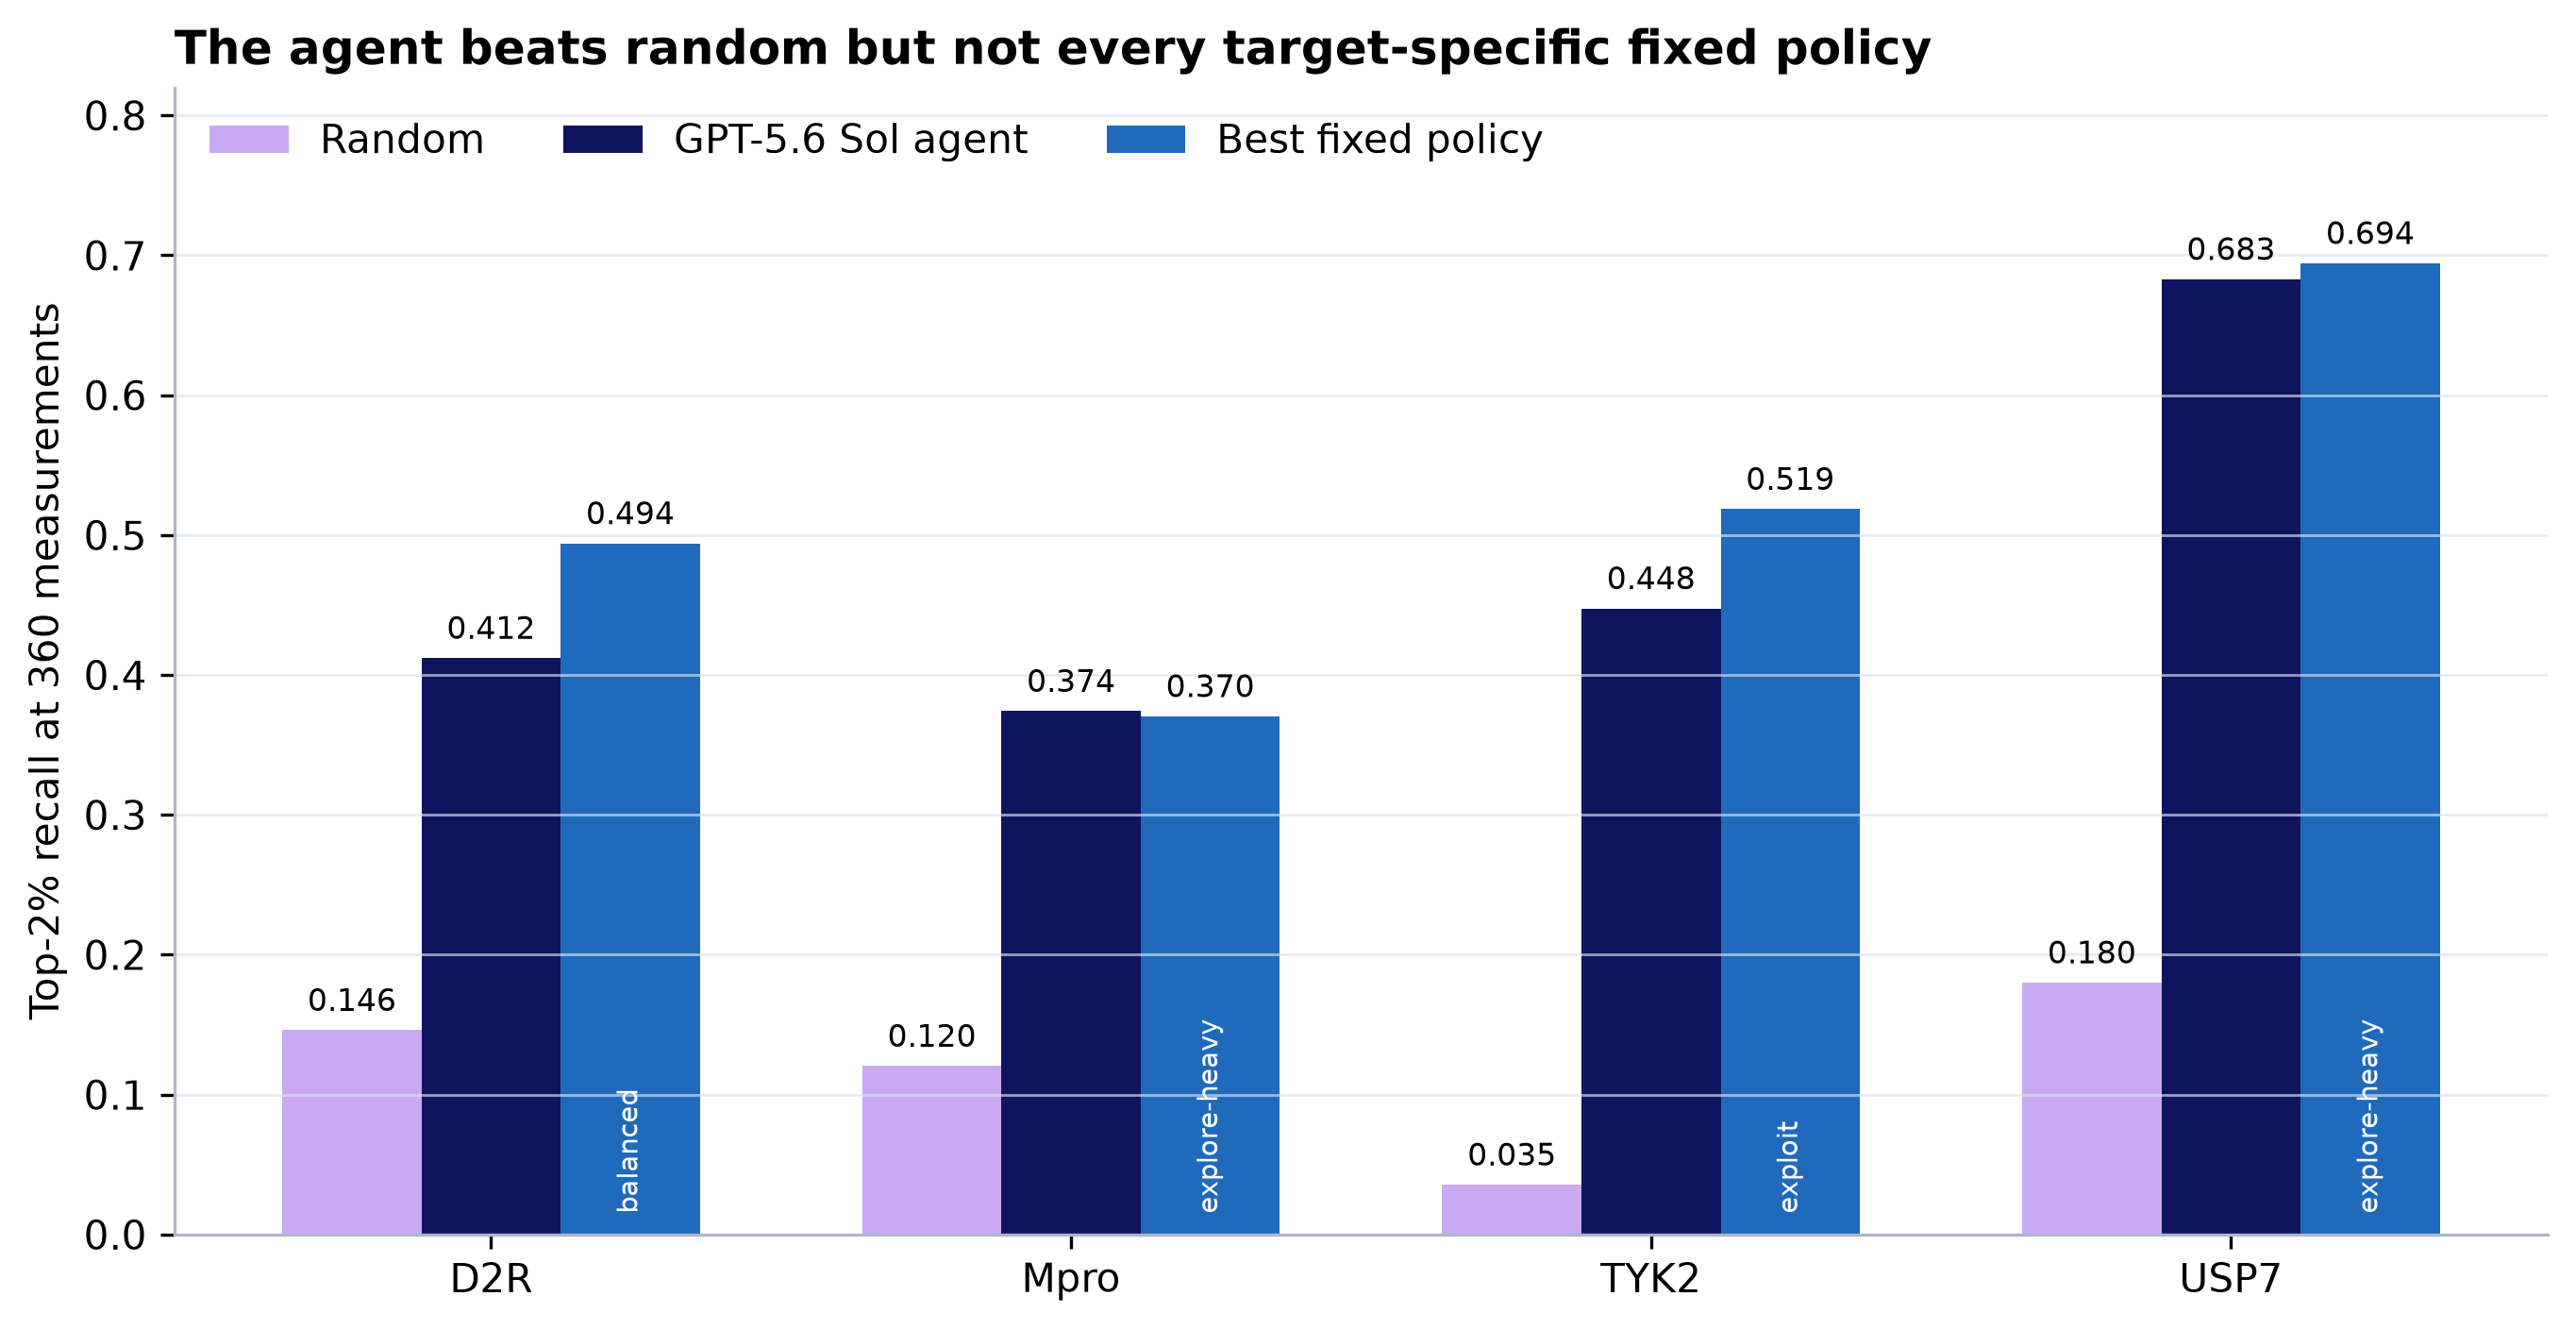
\includegraphics[width=\linewidth]{figures/endpoint_top2_comparison.png}
    \caption{Endpoint top-2\% recall after 360 measurements. Bars show means over ten paired seeds. The strongest fixed policy is selected separately for each target. The controller is uniformly better than random but not uniformly better than the target-specific leader.}
    \label{fig:endpoint}
\end{figure}

Against the strongest fixed policy, the result was heterogeneous (Table~\ref{tab:core}). D2R favored the balanced policy by 0.082 and TYK2 favored pure exploitation by 0.071; both paired intervals excluded zero. Mpro differed from explore-heavy by only +0.004 and USP7 differed from explore-heavy by -0.011, with both intervals crossing zero. The agent found the global-best compound in all Mpro, TYK2, and USP7 runs and seven of ten D2R runs.

\begin{table}[t]
\caption{Core endpoint comparison. Values are mean top-2\% recall; intervals describe the paired agent-minus-strongest-fixed difference.}
\label{tab:core}
\centering
\small
\begin{tabular}{lrrrrl}
\toprule
Target & Agent & Random & Best fixed & Difference & 95\% CI \\
\midrule
D2R  & .412 & .146 & .494 & -.082 & [-.150, -.020] \\
Mpro & .374 & .120 & .370 & +.004 & [-.013, +.017] \\
TYK2 & .448 & .036 & .519 & -.071 & [-.125, -.020] \\
USP7 & .683 & .180 & .694 & -.011 & [-.060, +.040] \\
\bottomrule
\end{tabular}
\end{table}

Learning curves show that the agent separated from random early and maintained that lead (Figure~\ref{fig:learning}). D2R and TYK2 developed persistent gaps relative to their target-specific fixed leaders, whereas Mpro and USP7 remained close for much of the budget. Endpoint recall therefore does not reflect a single anomalous final batch.

\begin{figure}[t]
    \centering
    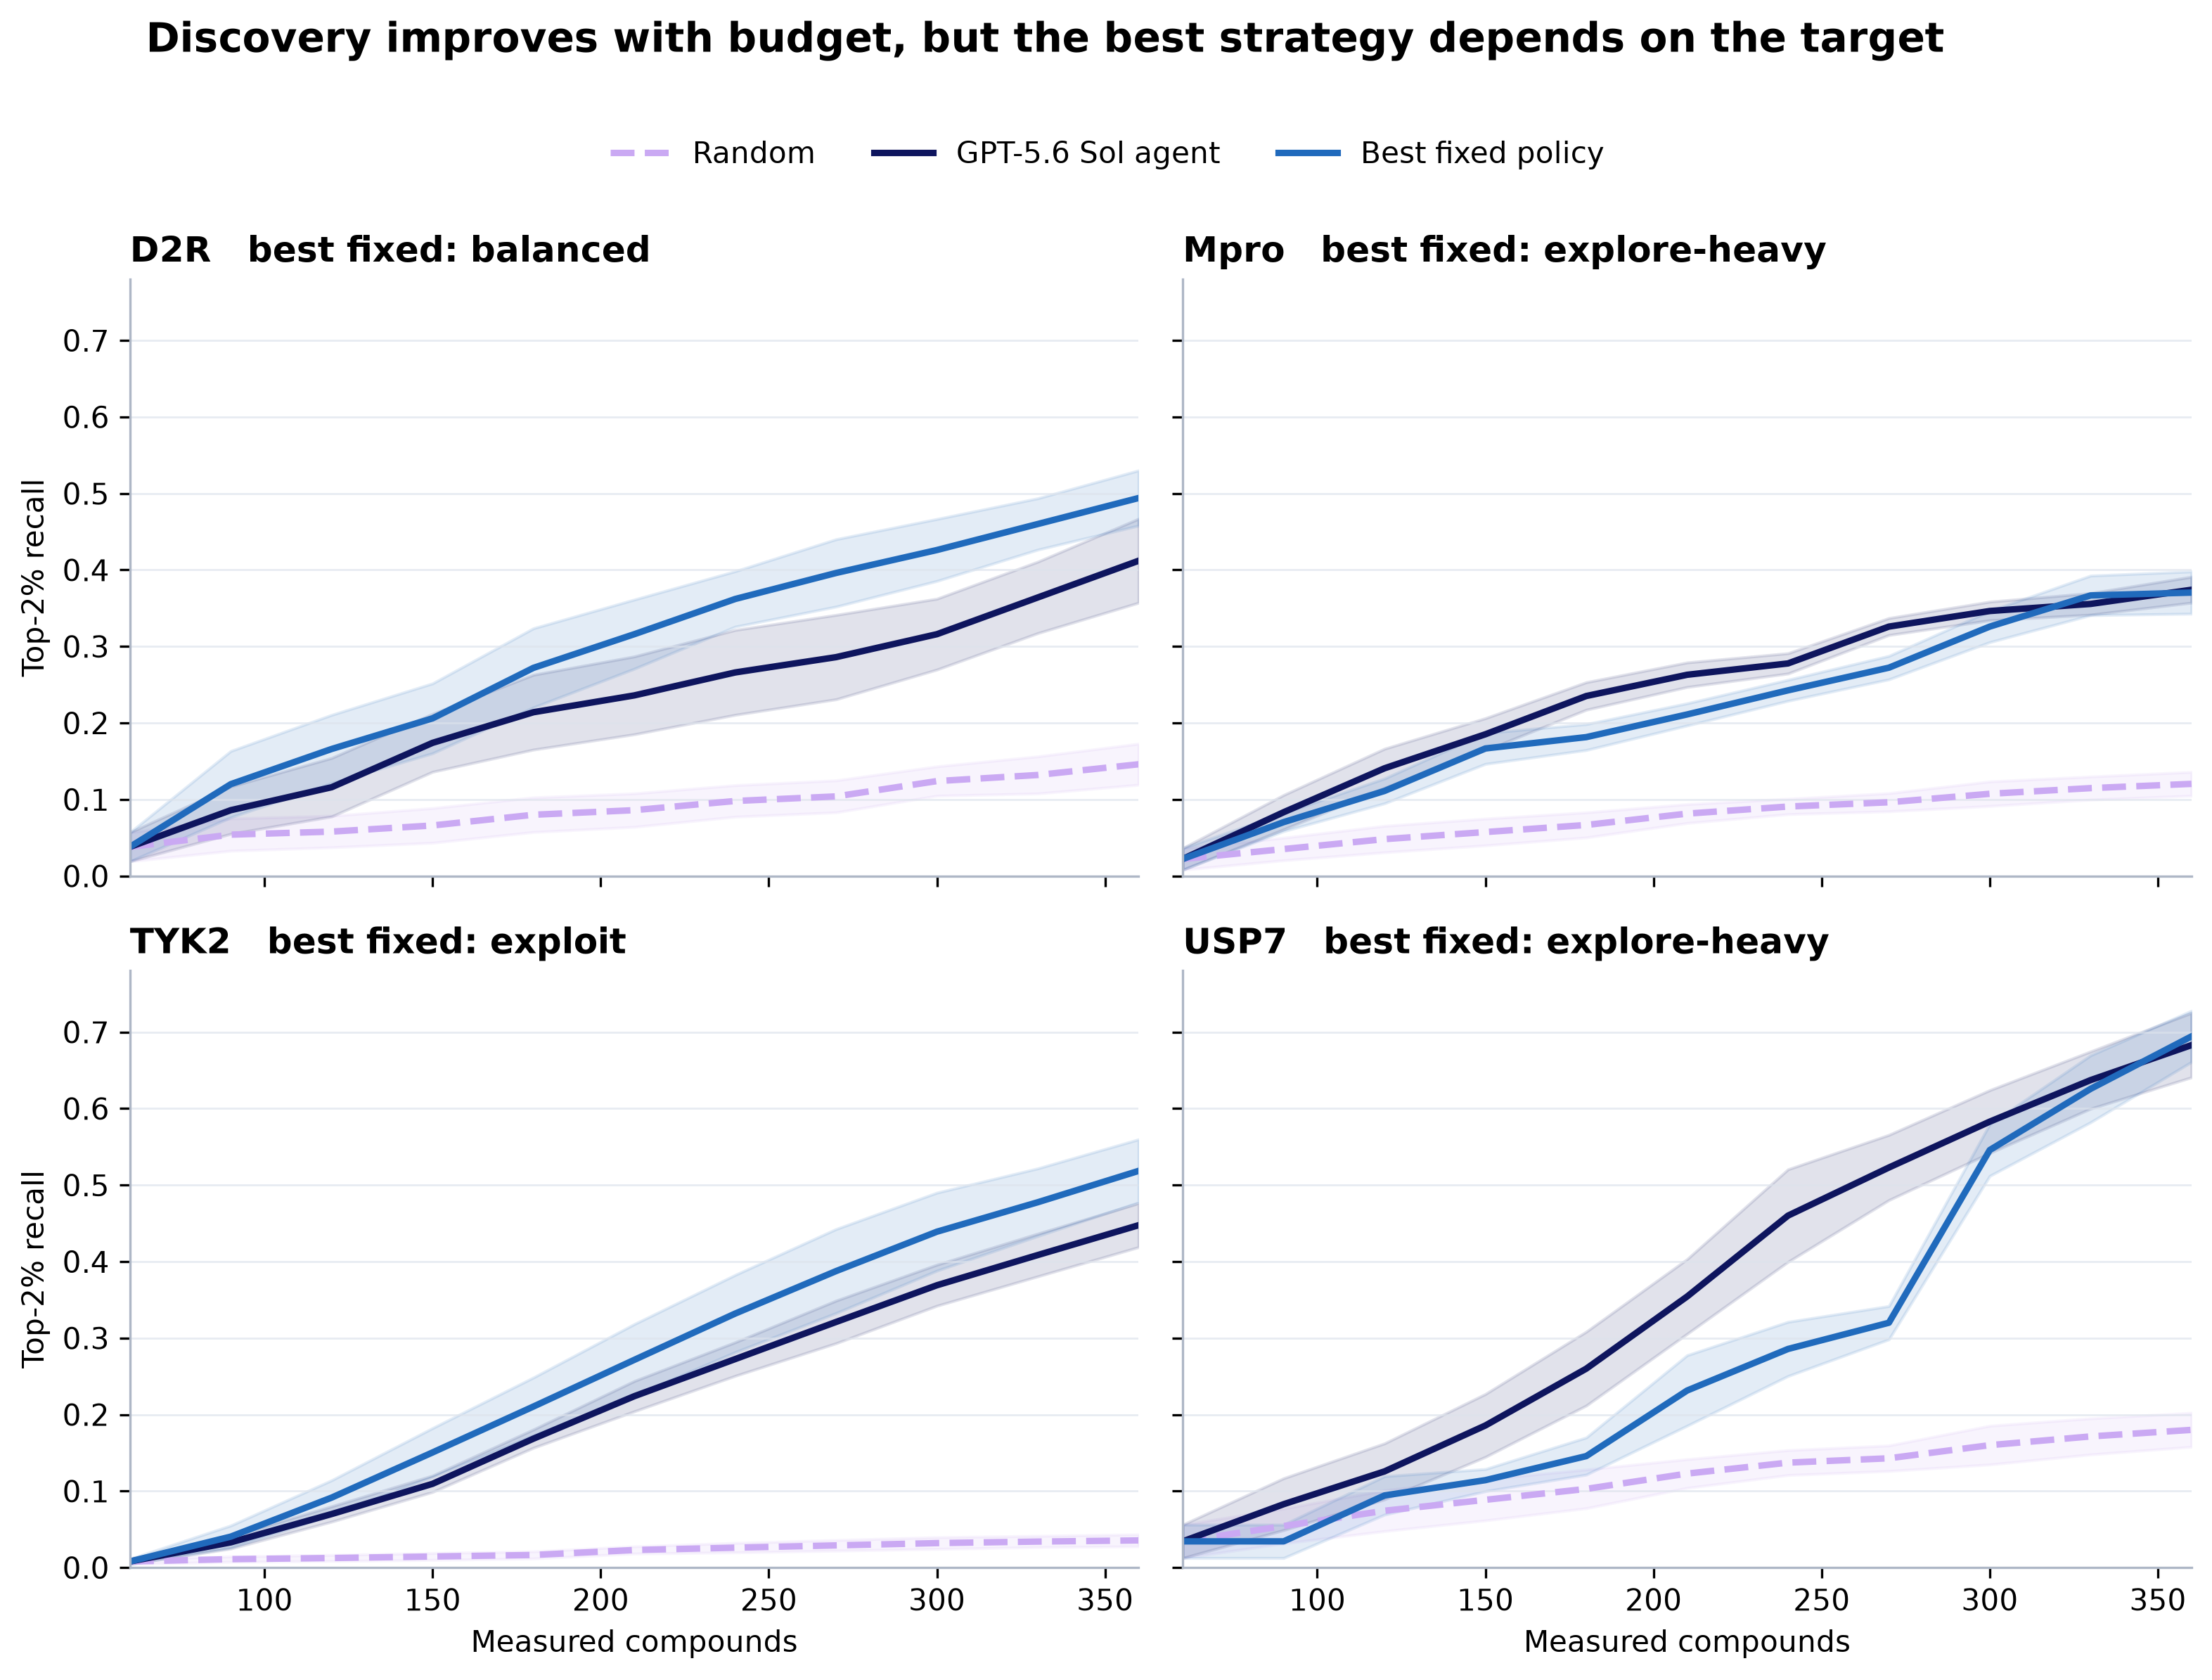
\includegraphics[width=\linewidth]{figures/top2_learning_curves.png}
    \caption{Top-2\% recall over the assay budget. Lines are means over ten seeds and bands are approximate 95\% confidence intervals based on the standard error.}
    \label{fig:learning}
\end{figure}

\subsection{Allocations adapt across targets and campaign stages}

The mean exploit allocation rose from 8.2 compounds in cycle 1 to 18.6 in cycle 10, while uncertainty fell from 11.6 to 6.7 and diversity from 10.2 to 4.7 (Figure~\ref{fig:alloc}). Target averages reveal distinct regimes: TYK2 was strongly exploitative (19.05 of 30 compounds per batch), Mpro emphasized uncertainty and diversity (5.80 exploit, 12.90 uncertain, 11.30 diverse), and D2R and USP7 used intermediate mixtures. Thus, the controller changed actions with both target and campaign stage. This behavioral adaptation does not establish that the natural-language rationale is a faithful causal explanation.

\begin{figure}[t]
    \centering
    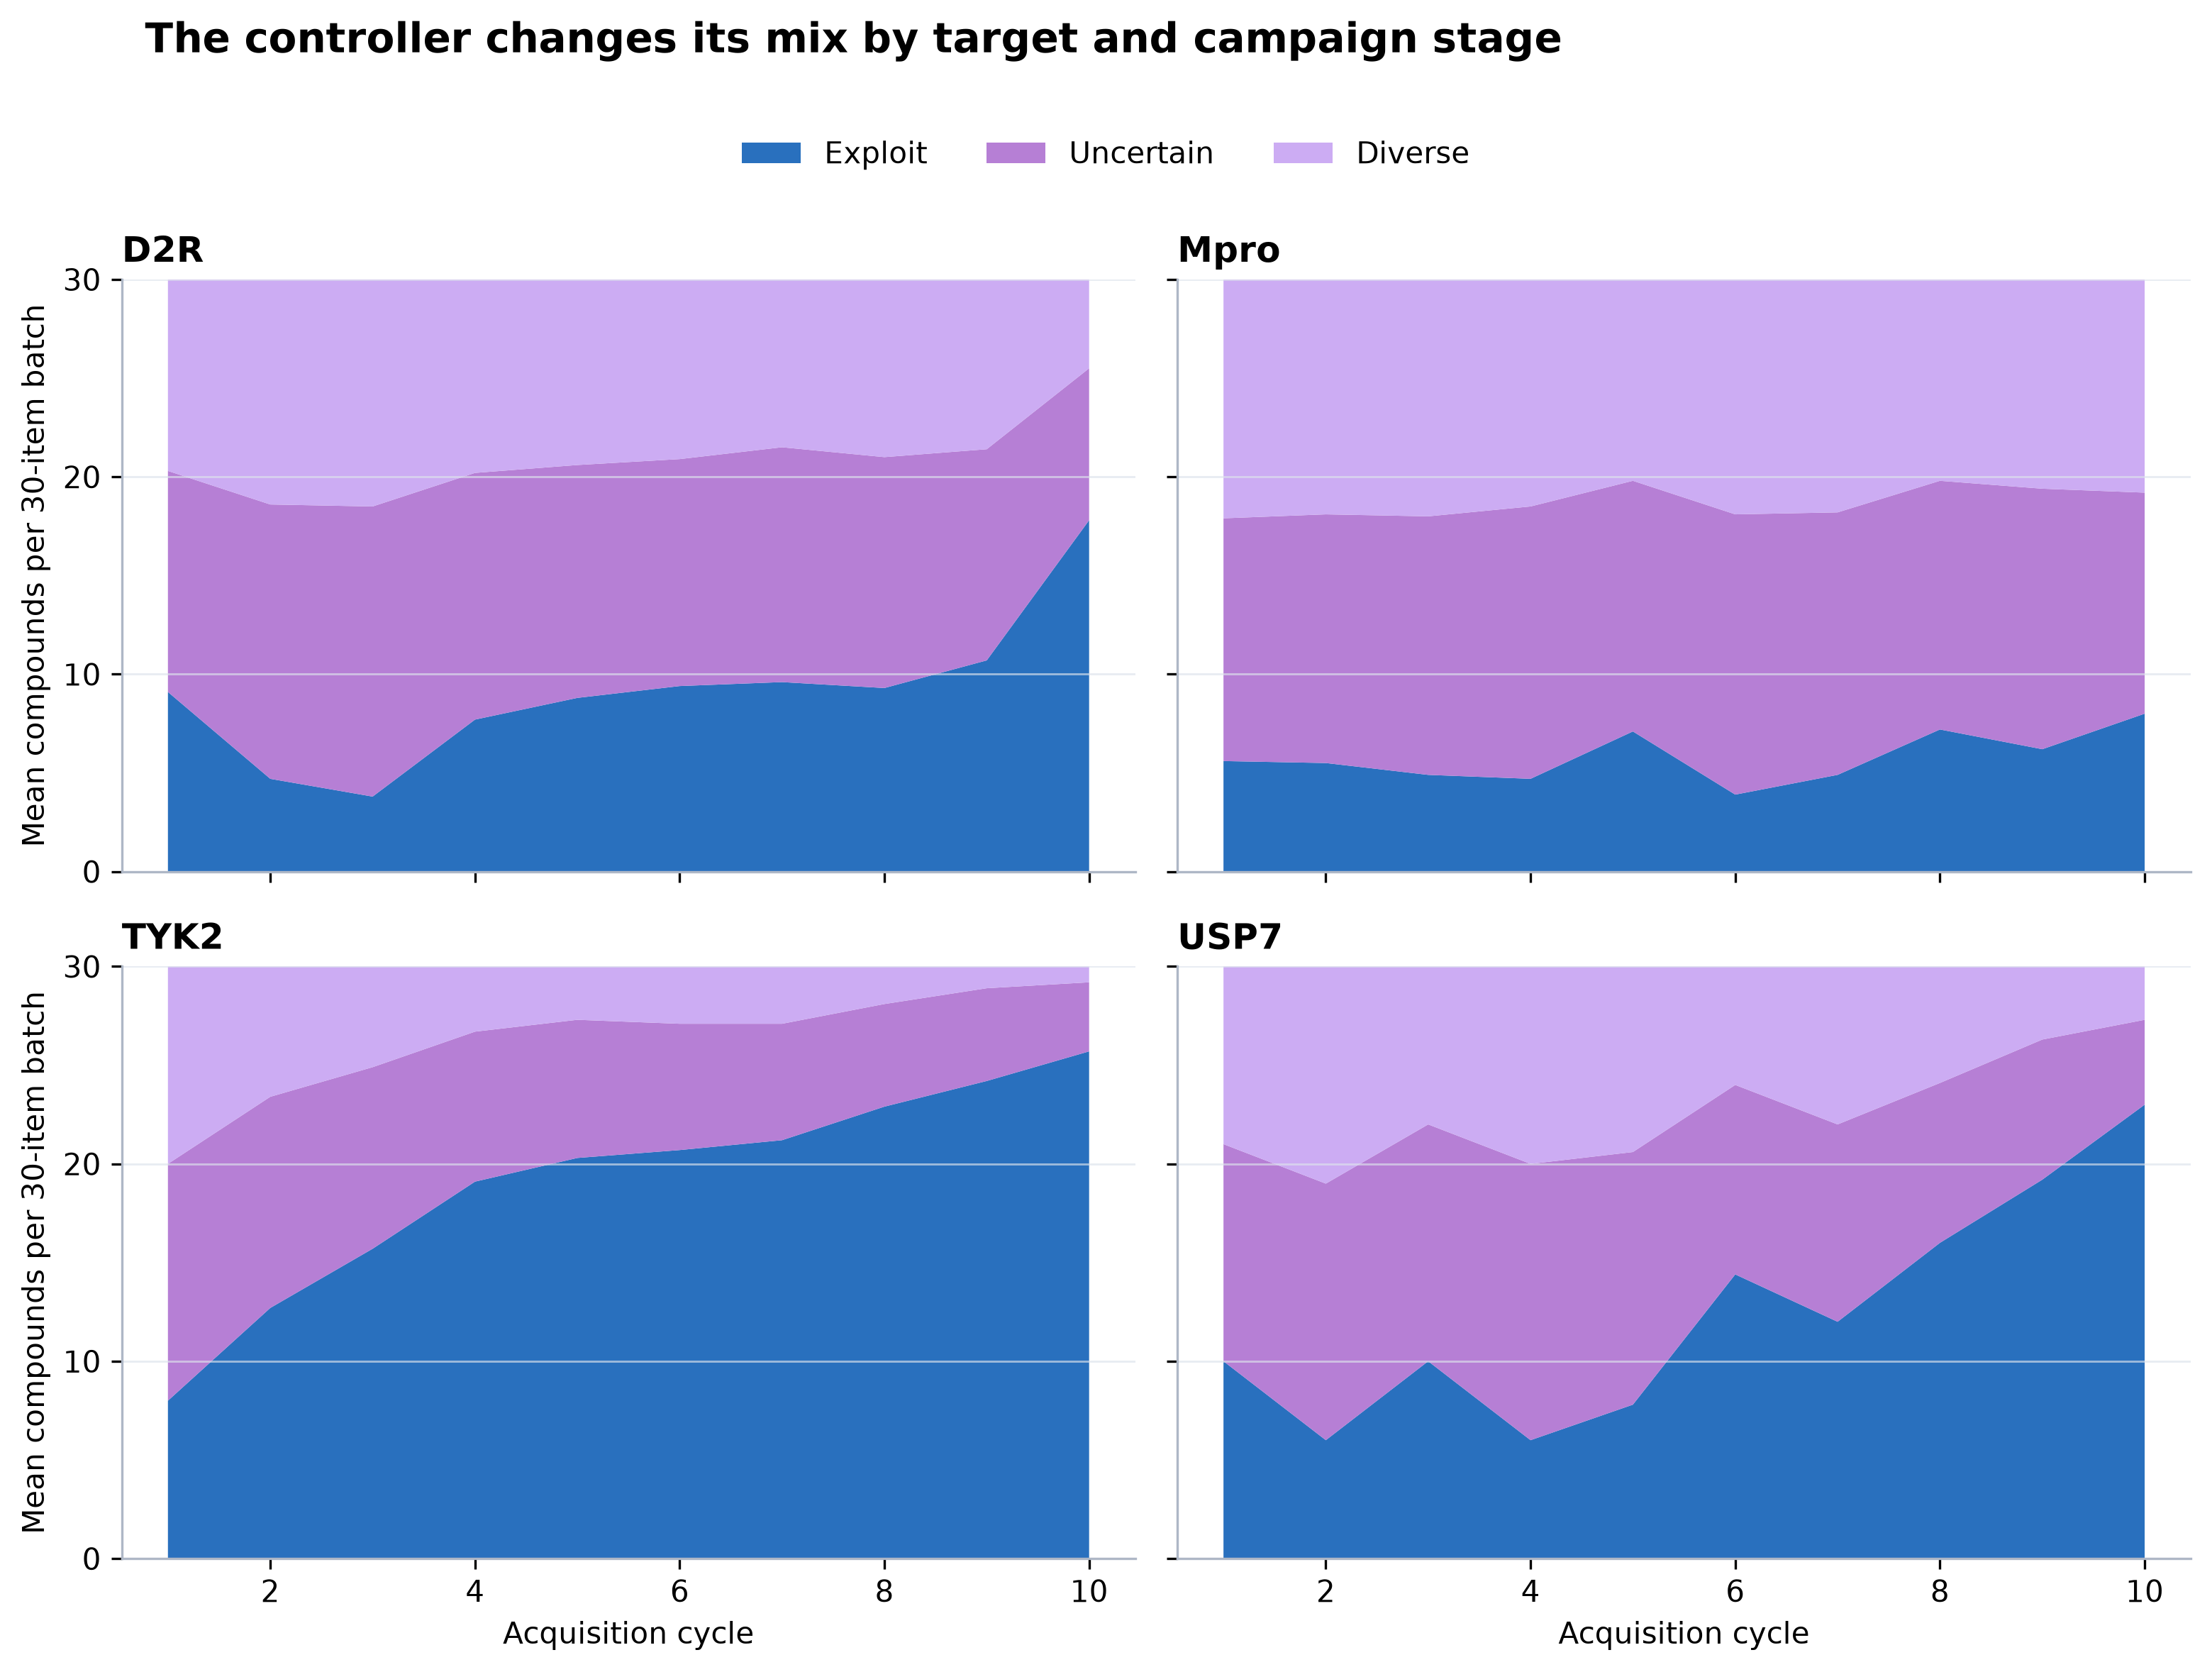
\includegraphics[width=\linewidth]{figures/agent_allocations_by_cycle.png}
    \caption{Mean composition of each 30-compound batch. Areas sum to 30. The controller generally moves from early information gathering toward late exploitation, with strong target dependence.}
    \label{fig:alloc}
\end{figure}

The comparison with all fixed policies further illustrates this heterogeneity (Figure~\ref{fig:heatmap}). The agent comfortably beat random, uncertainty-only, and several mismatched mixtures, but target-matched fixed policies remained difficult to beat. The heat map uses a single-hue Phthalo Blue scale with maximum color \texttt{\#0E155E}; signed cell labels retain which method is better.

\begin{figure}[t]
    \centering
    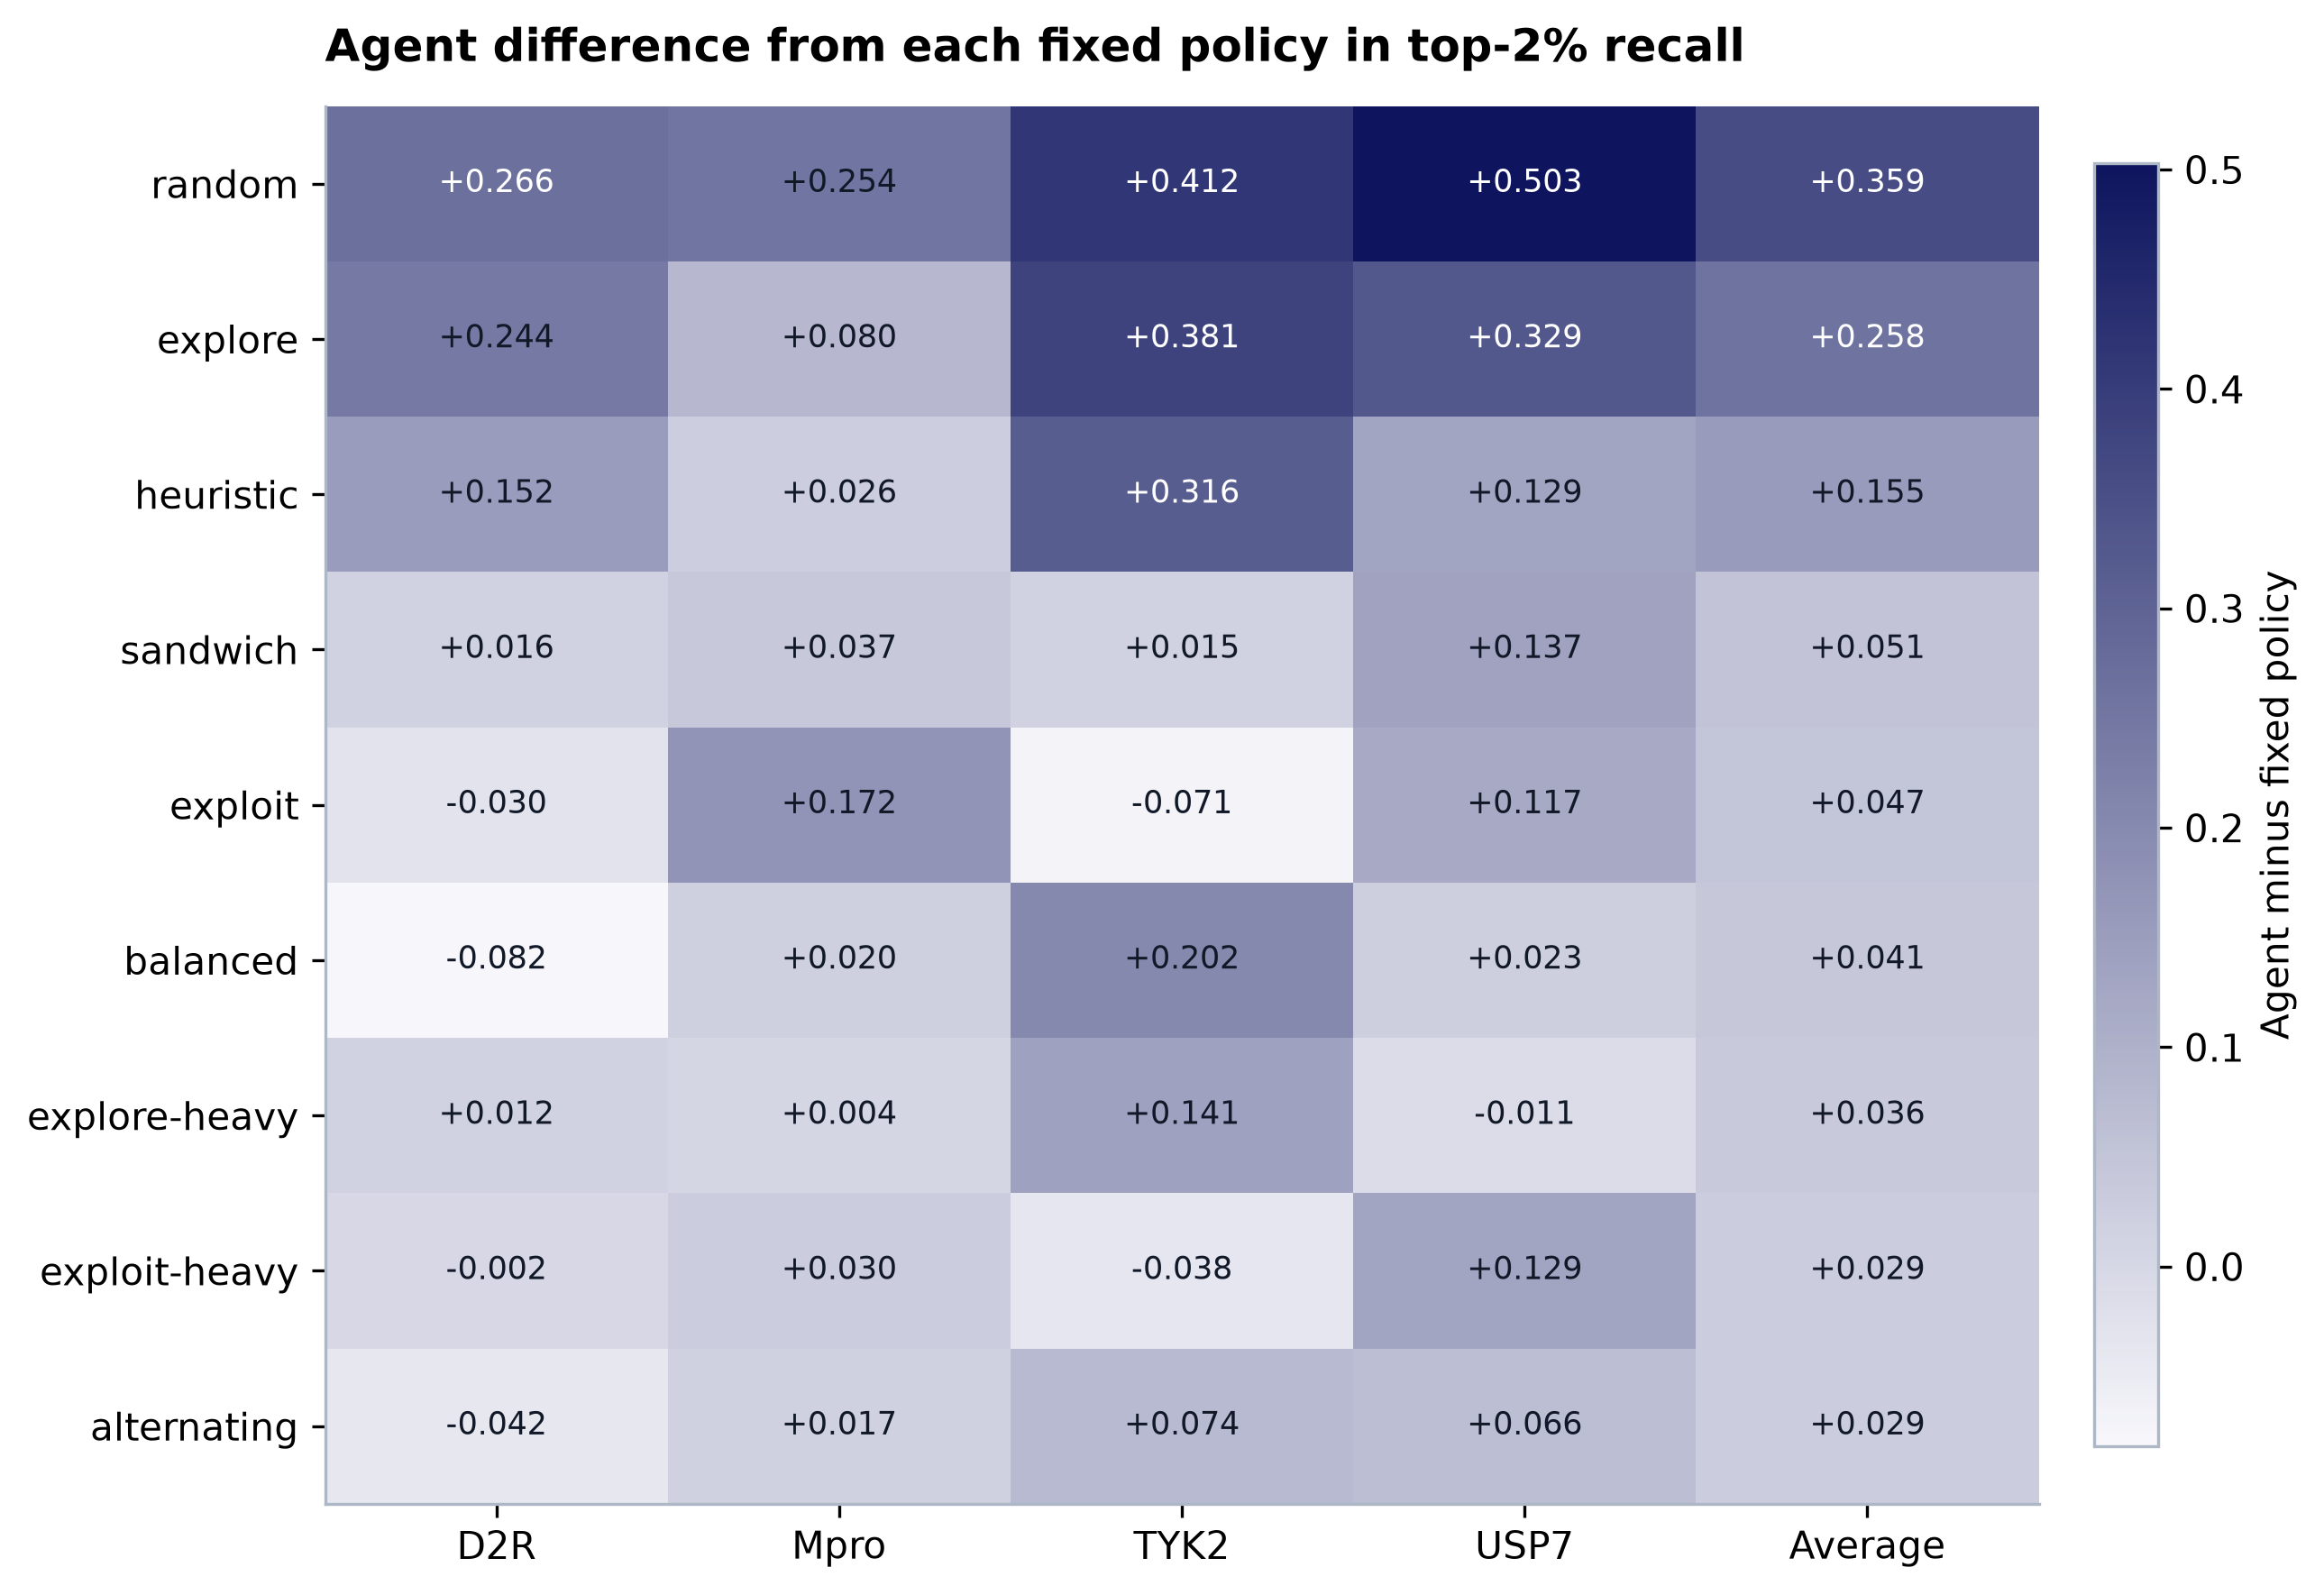
\includegraphics[width=\linewidth]{figures/agent_vs_policy_heatmap.png}
    \caption{Agent minus fixed-policy mean top-2\% recall. Positive values favor the controller. The average column is unweighted across targets and should be interpreted together with target-specific cells.}
    \label{fig:heatmap}
\end{figure}

\subsection{Expected outcomes are often correct when testable}

Of 400 expected outcomes, 321 contained at least one supported numerical threshold and 79 (19.75\%) were unscorable. The parser extracted 686 atomic claims, of which 86.30\% succeeded. The mean fraction of clauses satisfied was 87.28\%, while all clauses succeeded together in 71.65\% of scorable decisions. D2R and TYK2 were 100\% scorable, Mpro 83\%, and USP7 only 38\% because many USP7 forecasts were qualitative. This result shows that rationales can make testable claims, but it does not measure probability calibration.

\subsection{Information ablations have small endpoint effects}

Across 200 ablation campaigns, no single removed channel produced a large or universal loss (Figure~\ref{fig:ablation}). Removing diversity reduced D2R recall by 0.016 and was neutral or slightly positive elsewhere. Removing memory changed means by -0.004 to +0.004. Removing uncertainty improved D2R by 0.016, was nearly neutral on Mpro and TYK2, and reduced USP7 by 0.014. Shuffling evidence changed the mean by exactly zero on every target.

\begin{figure}[t]
    \centering
    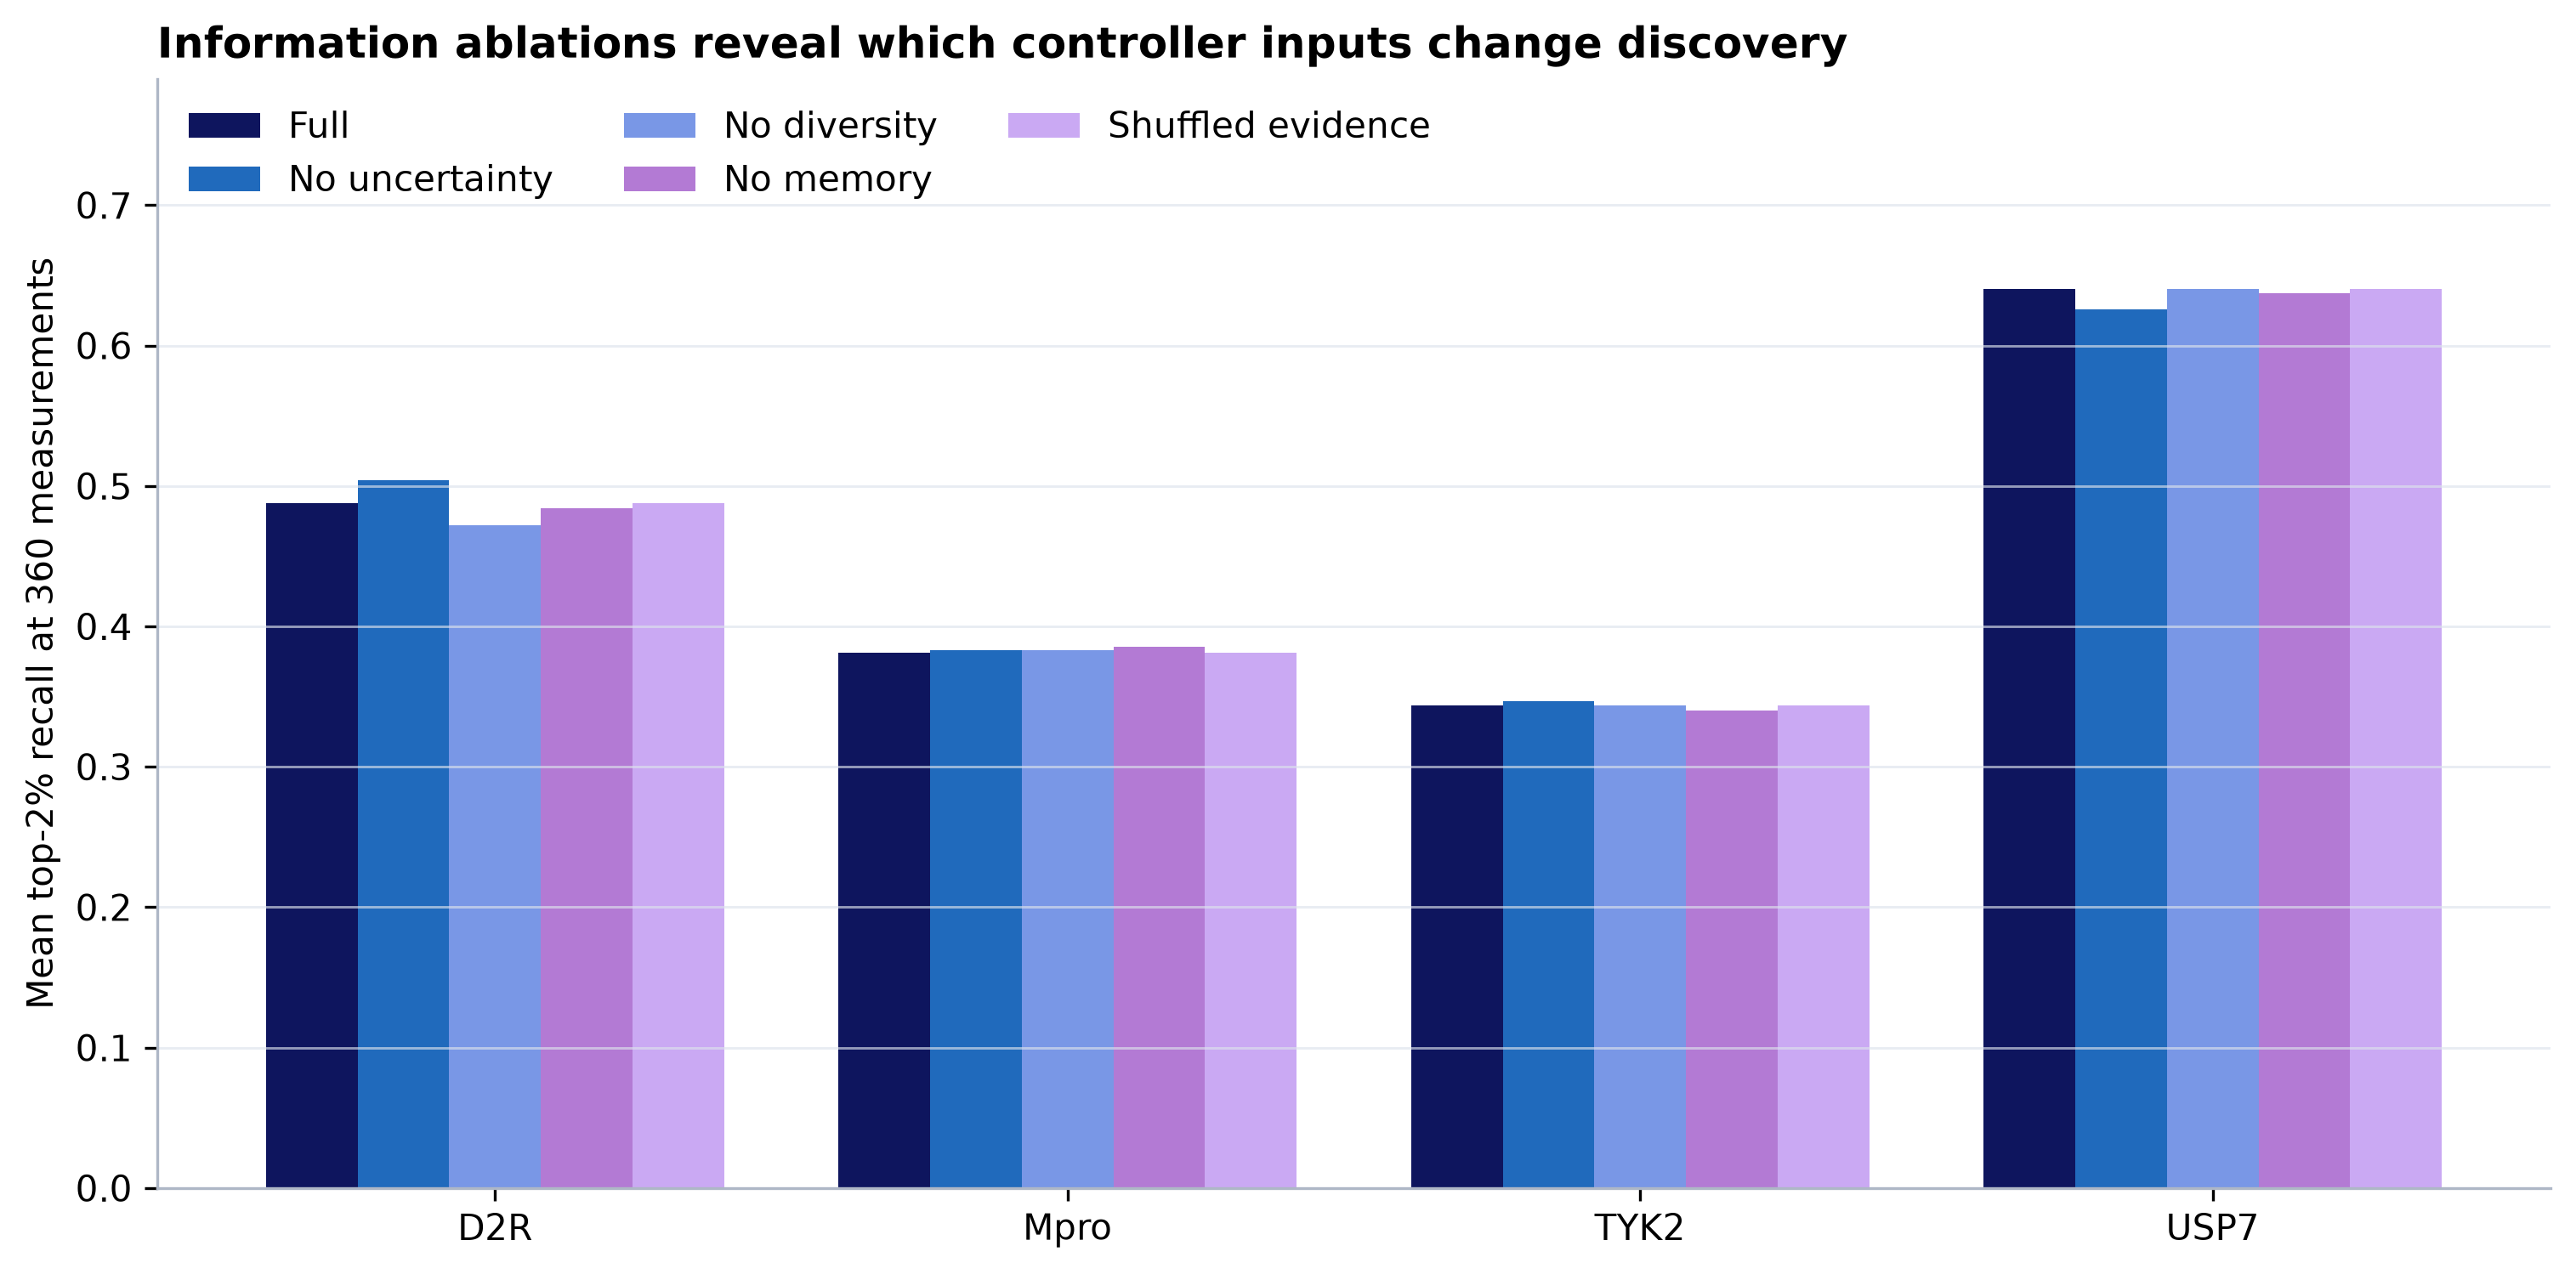
\includegraphics[width=\linewidth]{figures/information_ablation_endpoints.png}
    \caption{Mean endpoint top-2\% recall for the full-information rerun and four paired ablations. Differences are small and target-specific. Full-reference reruns are compared only with their paired ablation arms.}
    \label{fig:ablation}
\end{figure}

At the decision level, shuffled evidence produced the same allocation path as full information in all D2R, Mpro, and TYK2 campaigns and nine of ten USP7 campaigns. Therefore, fingerprint-bit identities in this evidence packet were usually unnecessary for the observed allocation. The ablation full-reference means differ from the core means because Codex task inference is not a frozen deterministic snapshot; only within-rerun paired comparisons have a causal interpretation.

\subsection{Availability constraints lower attainable recall}

An 80\% post-initial availability mask reduced agent top-2\% recall by 0.070 on D2R, 0.072 on Mpro, 0.114 on TYK2, and 0.069 on USP7 (Figure~\ref{fig:availability}). Under this constraint, the agent exceeded the strongest constrained fixed policy on Mpro and USP7 but remained behind on D2R and TYK2. The strongest fixed policies also lost recall relative to their unconstrained counterparts, confirming that access changes the problem rather than only disadvantaging the controller. Across 12,000 post-initial agent selections, no unavailable compound was selected.

\begin{figure}[t]
    \centering
    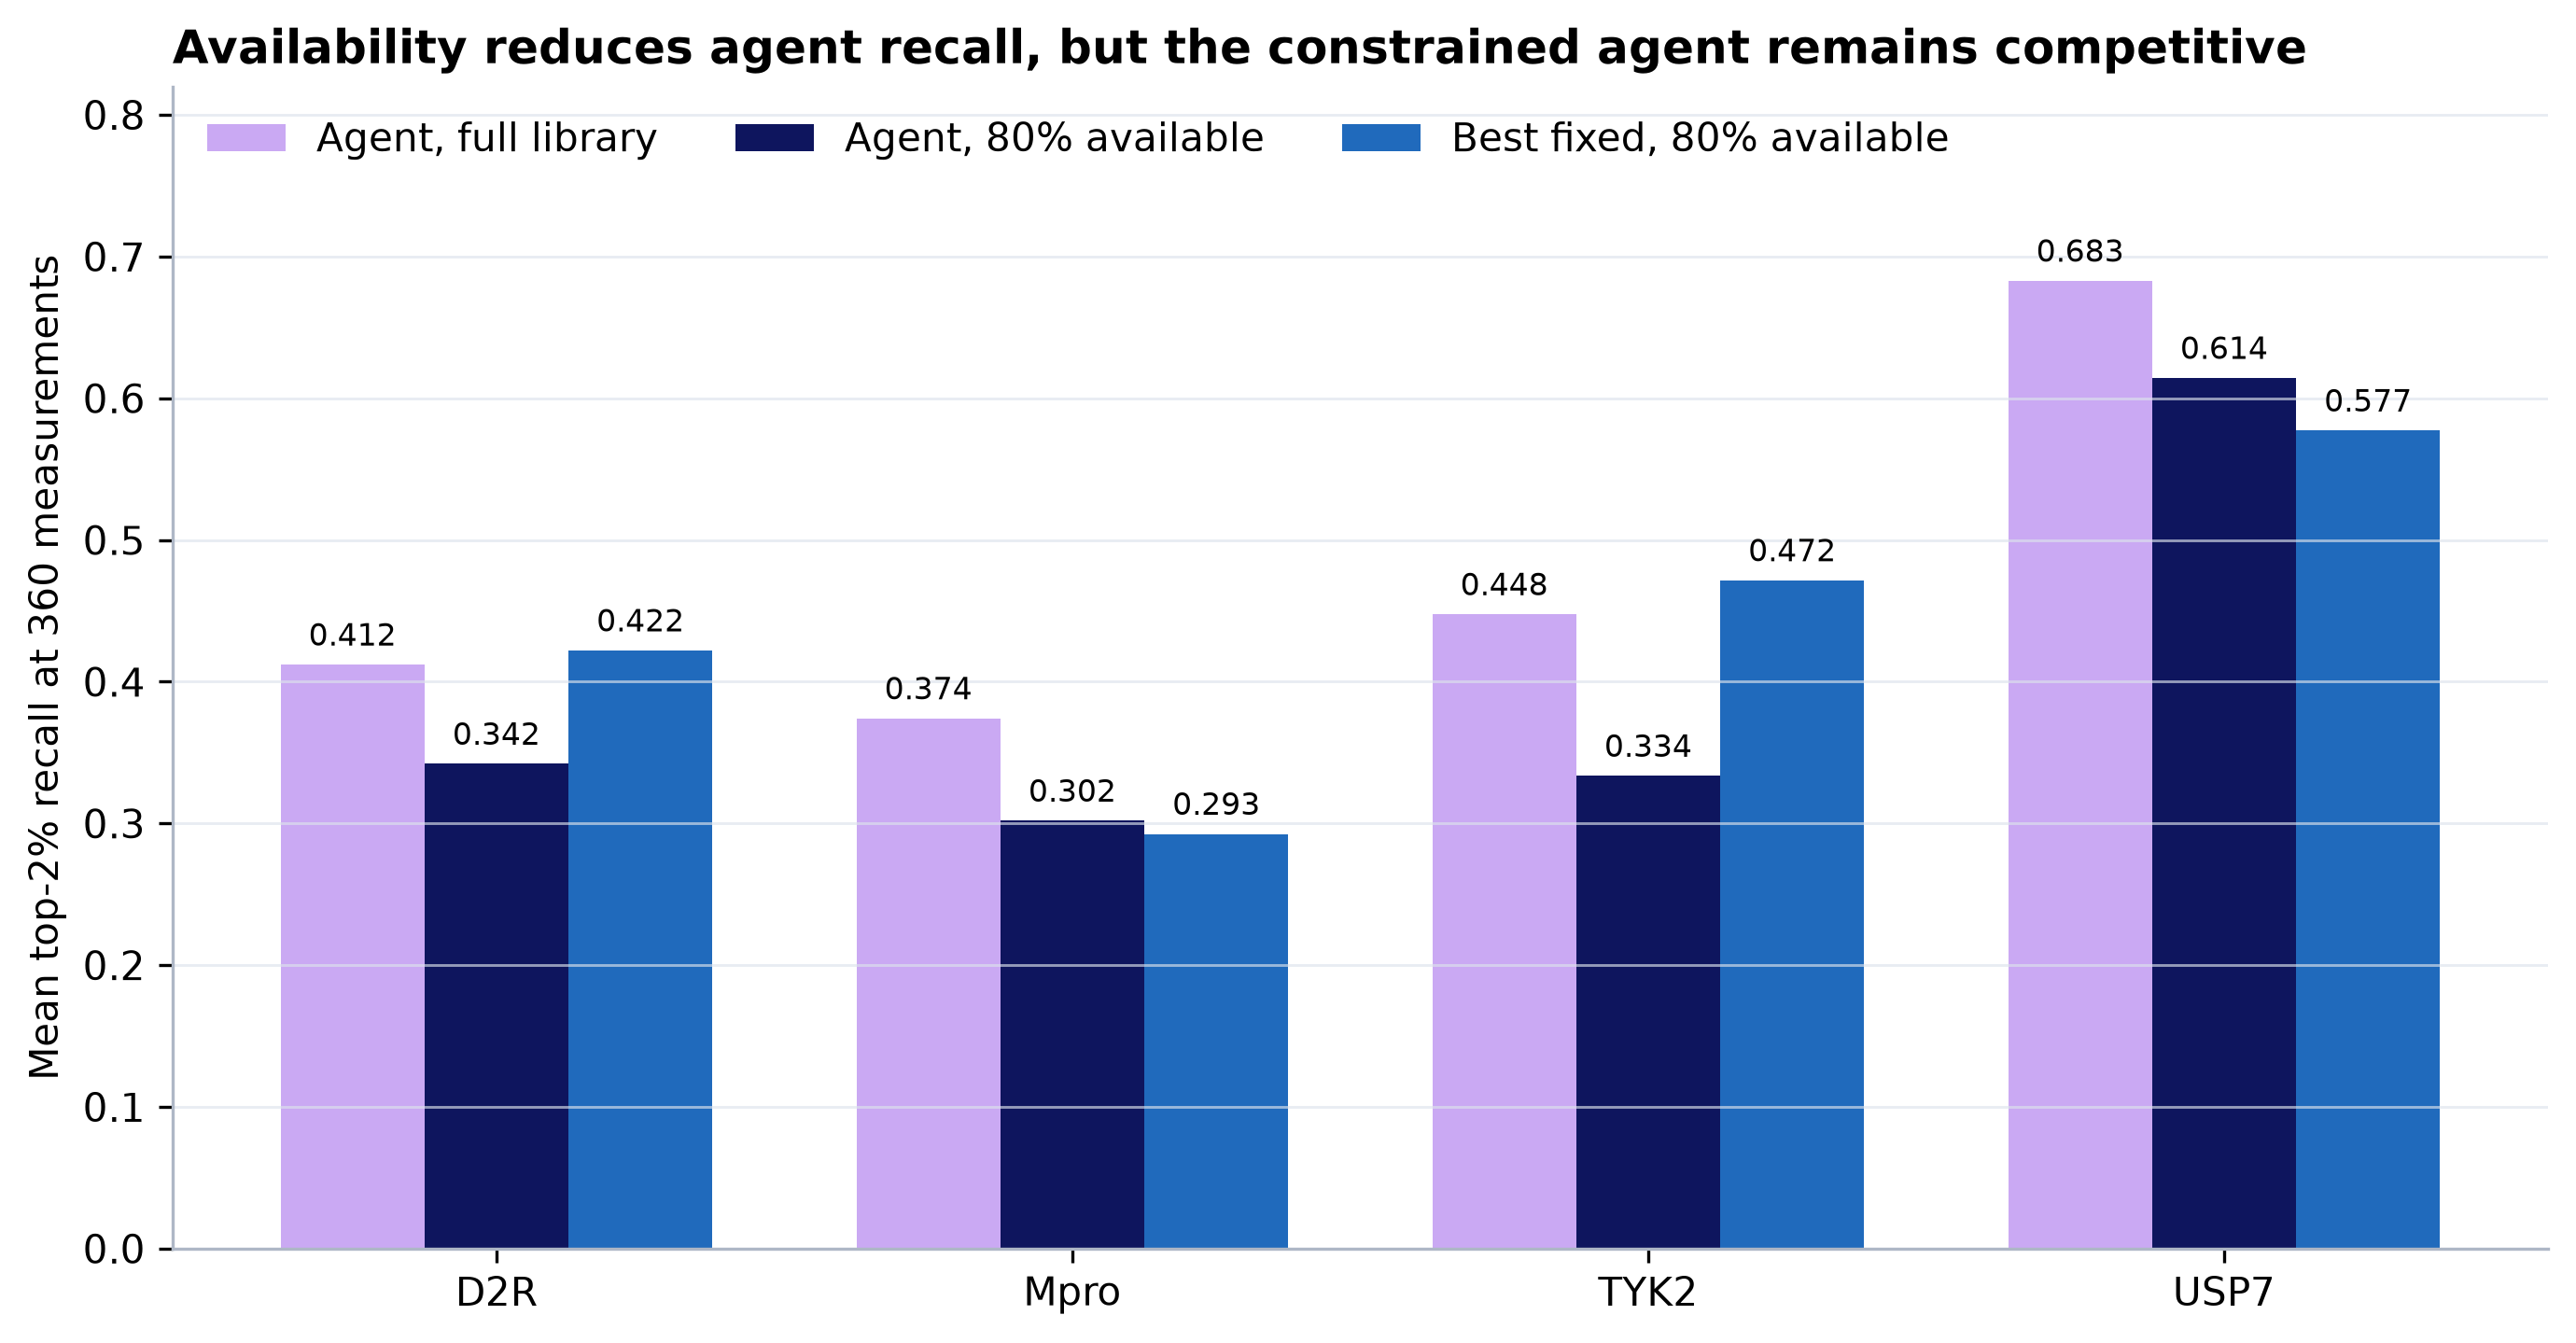
\includegraphics[width=\linewidth]{figures/availability_agent_comparison.png}
    \caption{Mean endpoint top-2\% recall for the unconstrained agent, the 80\%-availability agent, and the strongest constrained fixed policy. Each bar averages ten paired seeds.}
    \label{fig:availability}
\end{figure}

\section{Discussion}

The benchmark supports three conclusions. First, language-model strategy control is useful: it beat random in every matched campaign, respected every batch constraint, and found the global optimum reliably on three targets. Second, adaptation is not the same as dominance. Target-specific fixed policies were better on D2R and TYK2, and the controller's allocations reveal why: TYK2 rewarded aggressive exploitation, while D2R favored a stable balanced mixture. Third, explanation channels require causal testing. High threshold-claim success shows that rationales can be empirically checked, but the shuffled-evidence ablation shows that one ostensibly explanatory channel rarely changed actions.

These findings argue for controllers that are evaluated as decision policies rather than judged from fluent rationales. A practical controller should state quantitative predictions, expose its allocation, obey feasibility constraints, and be compared with strong target-specific policies. Future versions should emit probabilities for formal calibration and use a frozen versioned API snapshot when exact replication and token accounting are required.

\paragraph{Limitations.}
The study is retrospective and uses known affinity labels as a virtual assay; it does not model wet-lab noise, synthesis time, procurement cost, or assay failure. The GP, Tanimoto kernel, and fingerprint representation are fixed for fairness, so conclusions may change with other surrogates. Codex-task inference is not an exact model snapshot. The threshold scorer captures explicit templates but not every qualitative claim. Finally, four targets are enough to expose heterogeneity but not to establish broad generality.

\paragraph{Potential impact.}
Better allocation can reduce unnecessary screening, but virtual performance can be mistaken for prospective evidence. The controller should not be used to prioritize real compounds without domain review, experimental validation, safety assessment, and access controls appropriate to dual-use chemistry.

\section{Conclusion}

A language-model controller can successfully allocate exploit, uncertainty, and diversity queues during batch ligand discovery. It consistently improves over random sampling and can match the strongest fixed policy on some targets, but it is not universally superior. Paired ablations and availability constraints show that both information use and operational access must be tested directly. The most defensible role for the language model is therefore an auditable strategy layer inside a numerically controlled active-learning system.

\bibliographystyle{plainnat}
\bibliography{references}

\appendix

\section{Additional endpoint results}

\begin{figure}[h]
    \centering
    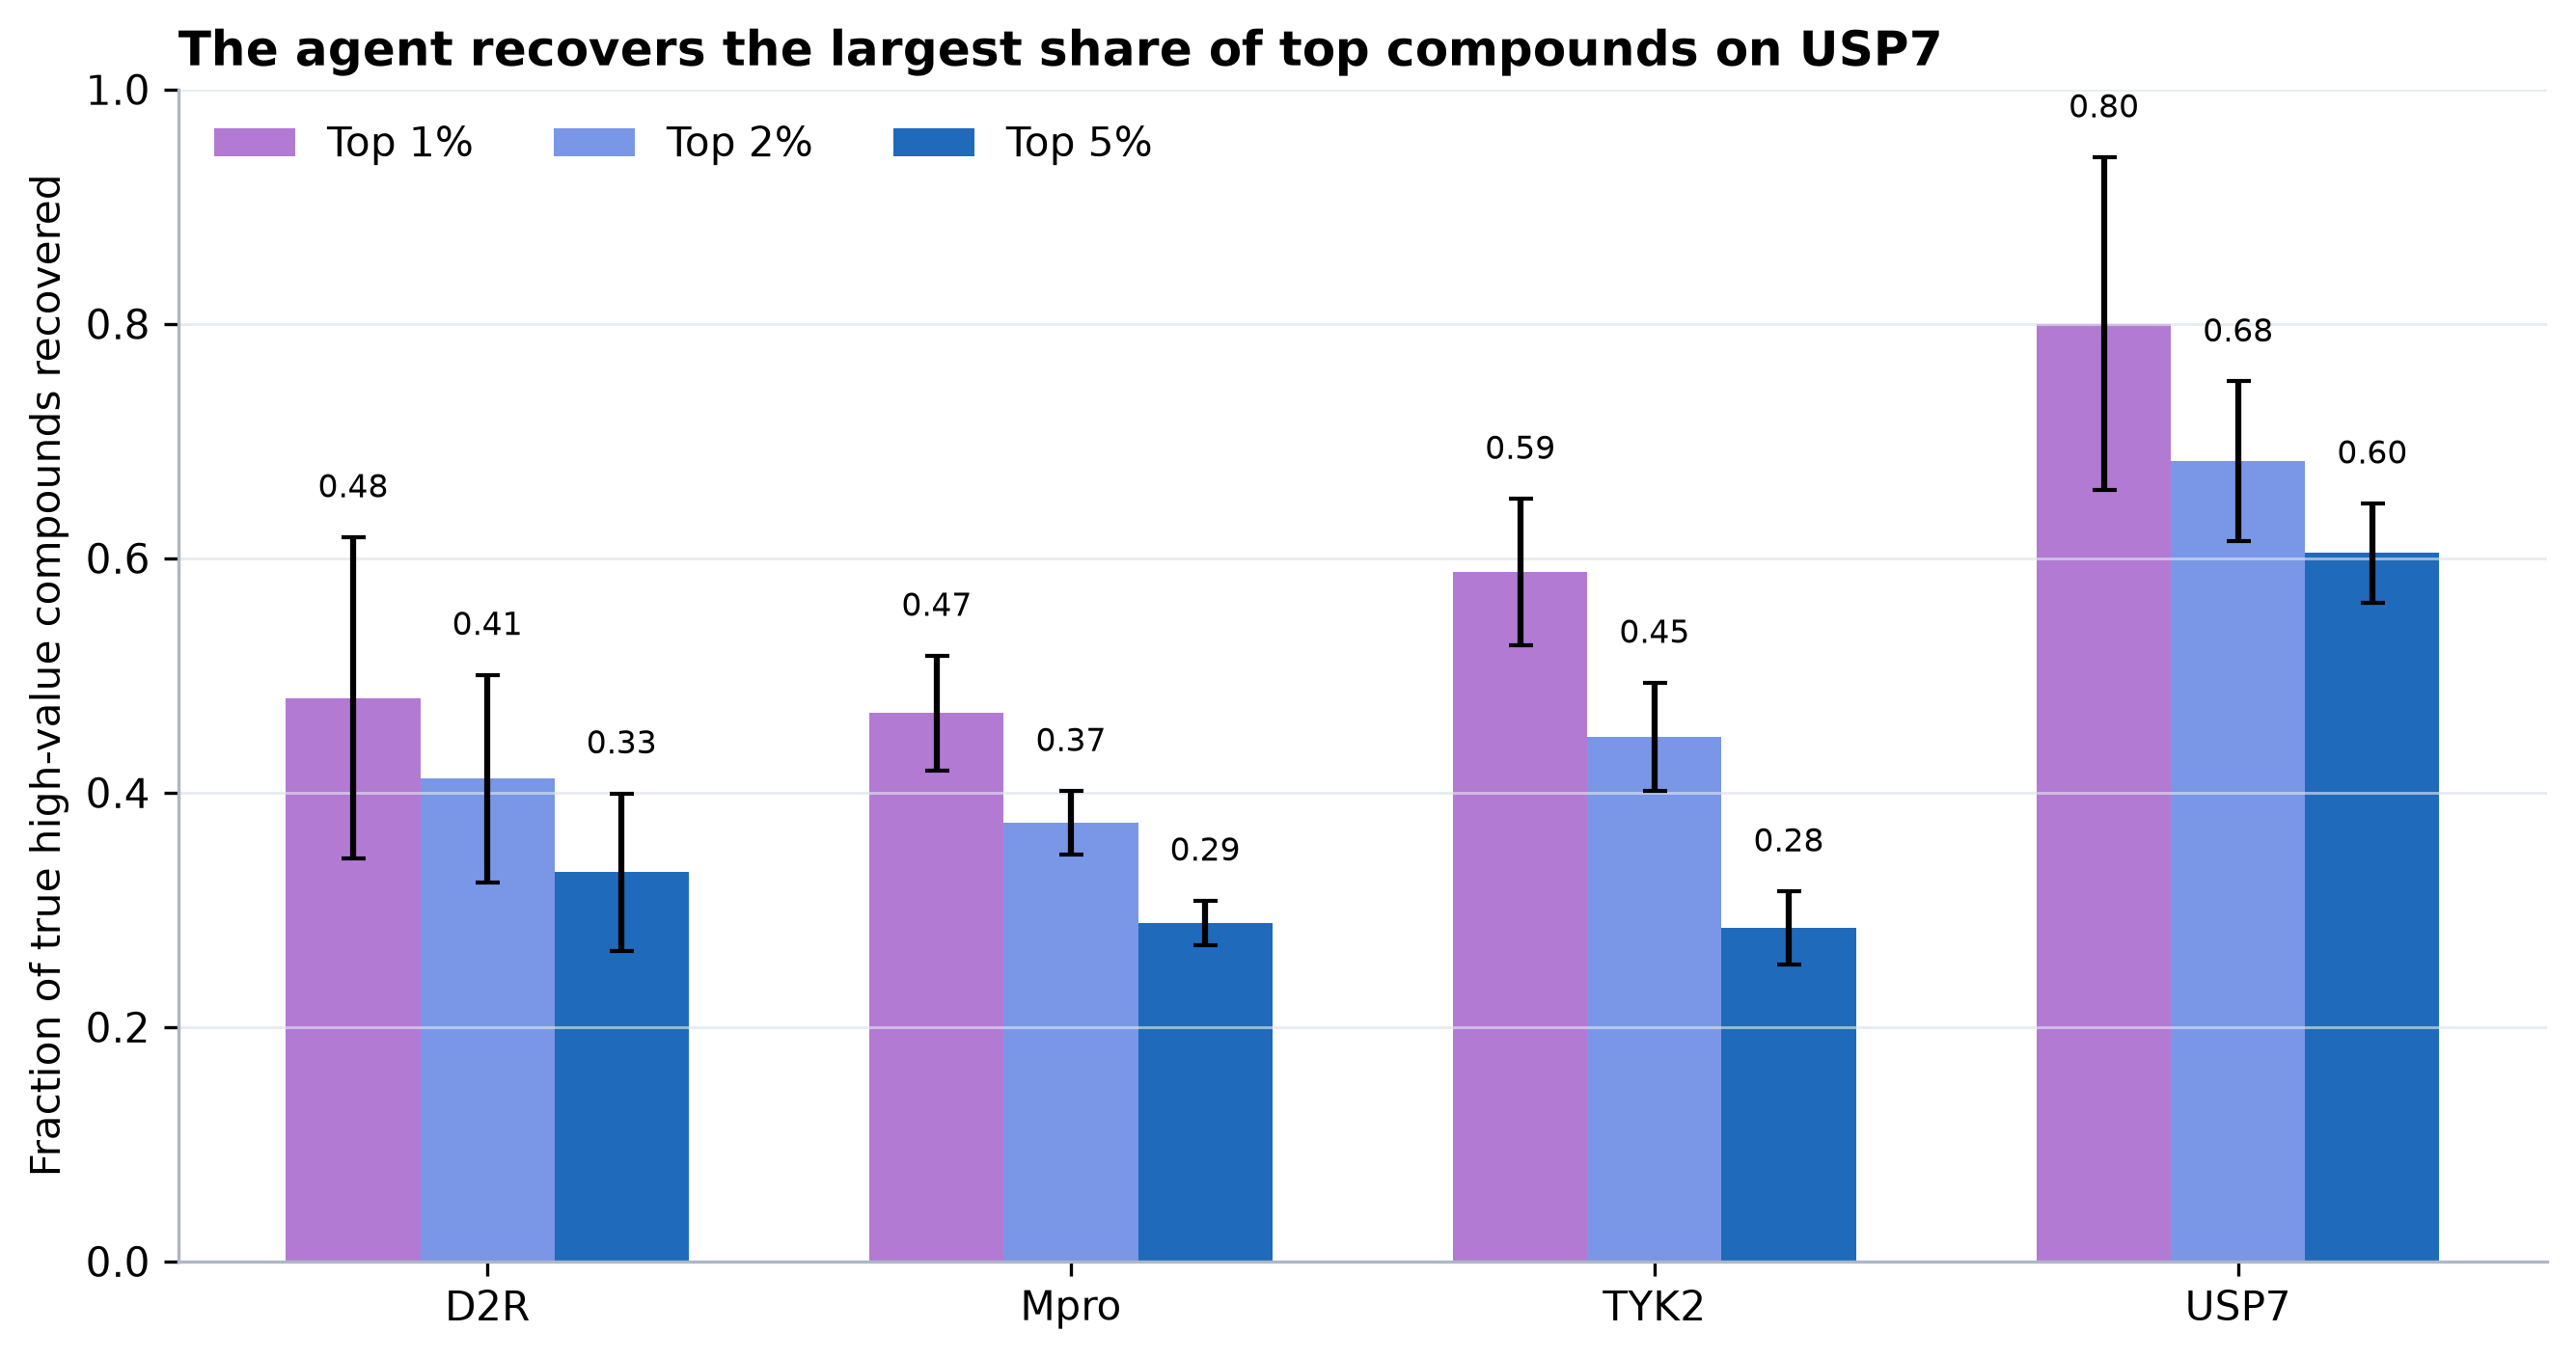
\includegraphics[width=\linewidth]{figures/endpoint_recall_levels.png}
    \caption{Agent endpoint recall at the top-1\%, top-2\%, and top-5\% thresholds. Error bars show standard deviation over ten seeds.}
\end{figure}

\section{Forecast scoring detail}

\begin{figure}[h]
    \centering
    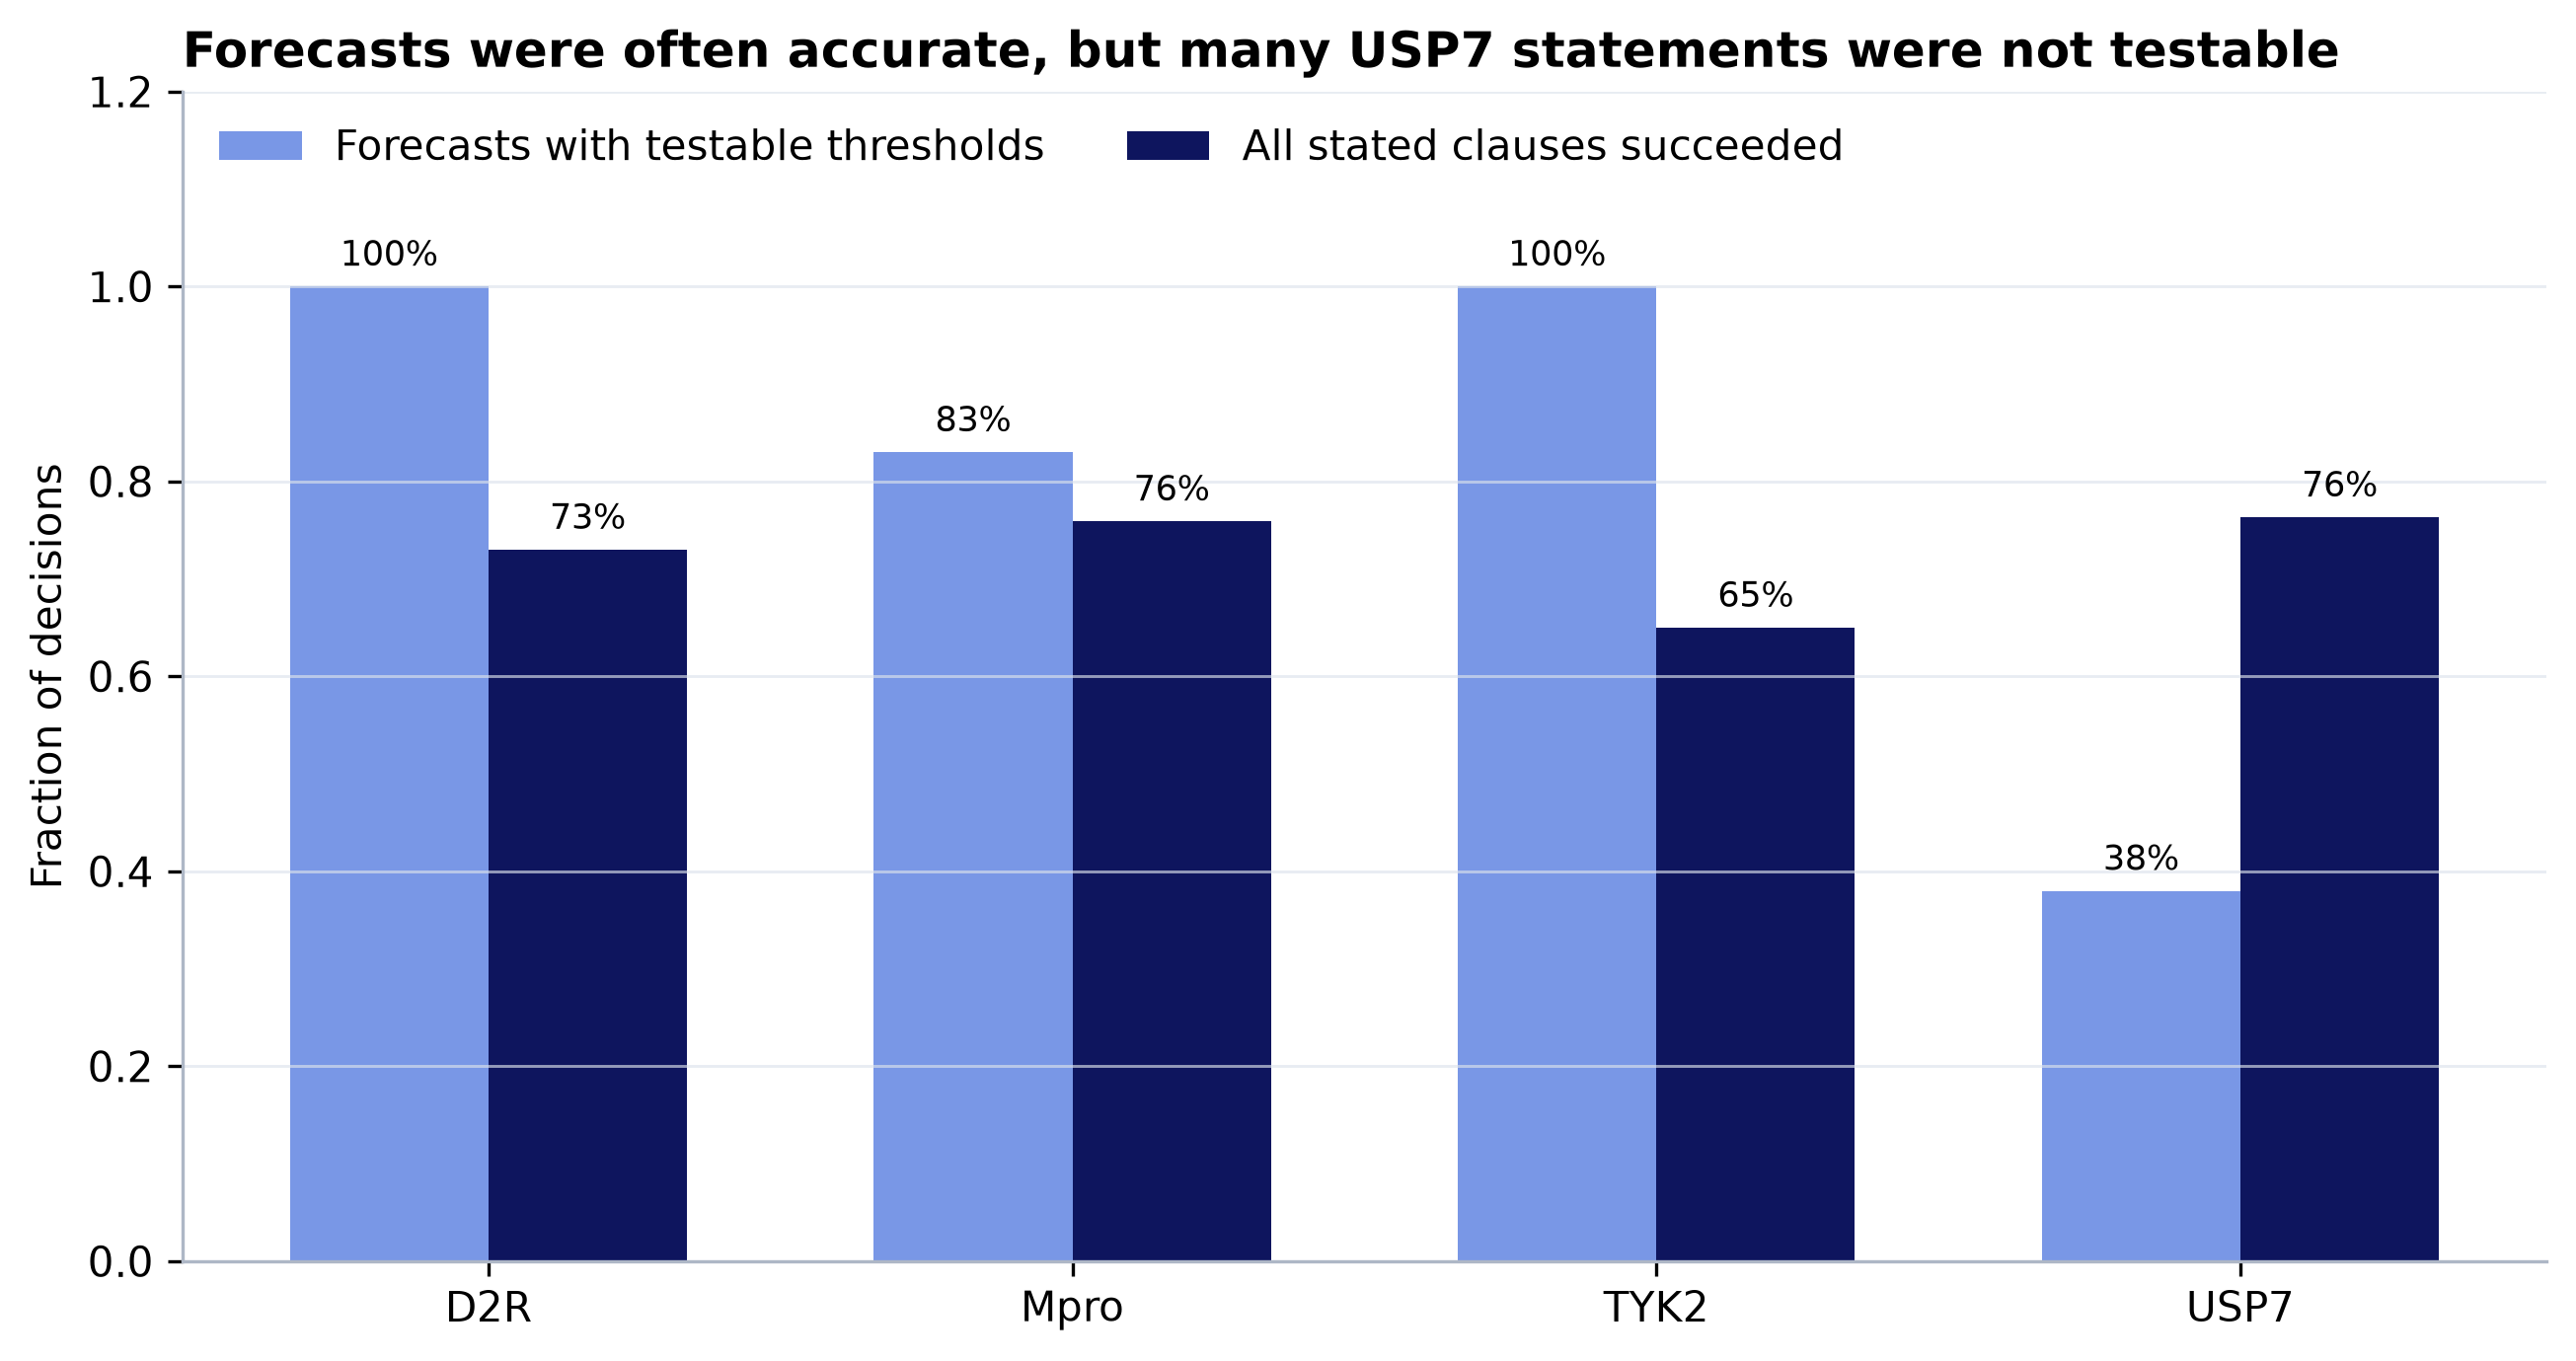
\includegraphics[width=\linewidth]{figures/forecast_testability_and_success.png}
    \caption{Forecast testability and conjunction success by target. Low USP7 testability reflects qualitative wording, not necessarily worse numeric claims among the scorable subset.}
\end{figure}

\section{Fixed policies under availability constraints}

\begin{figure}[h]
    \centering
    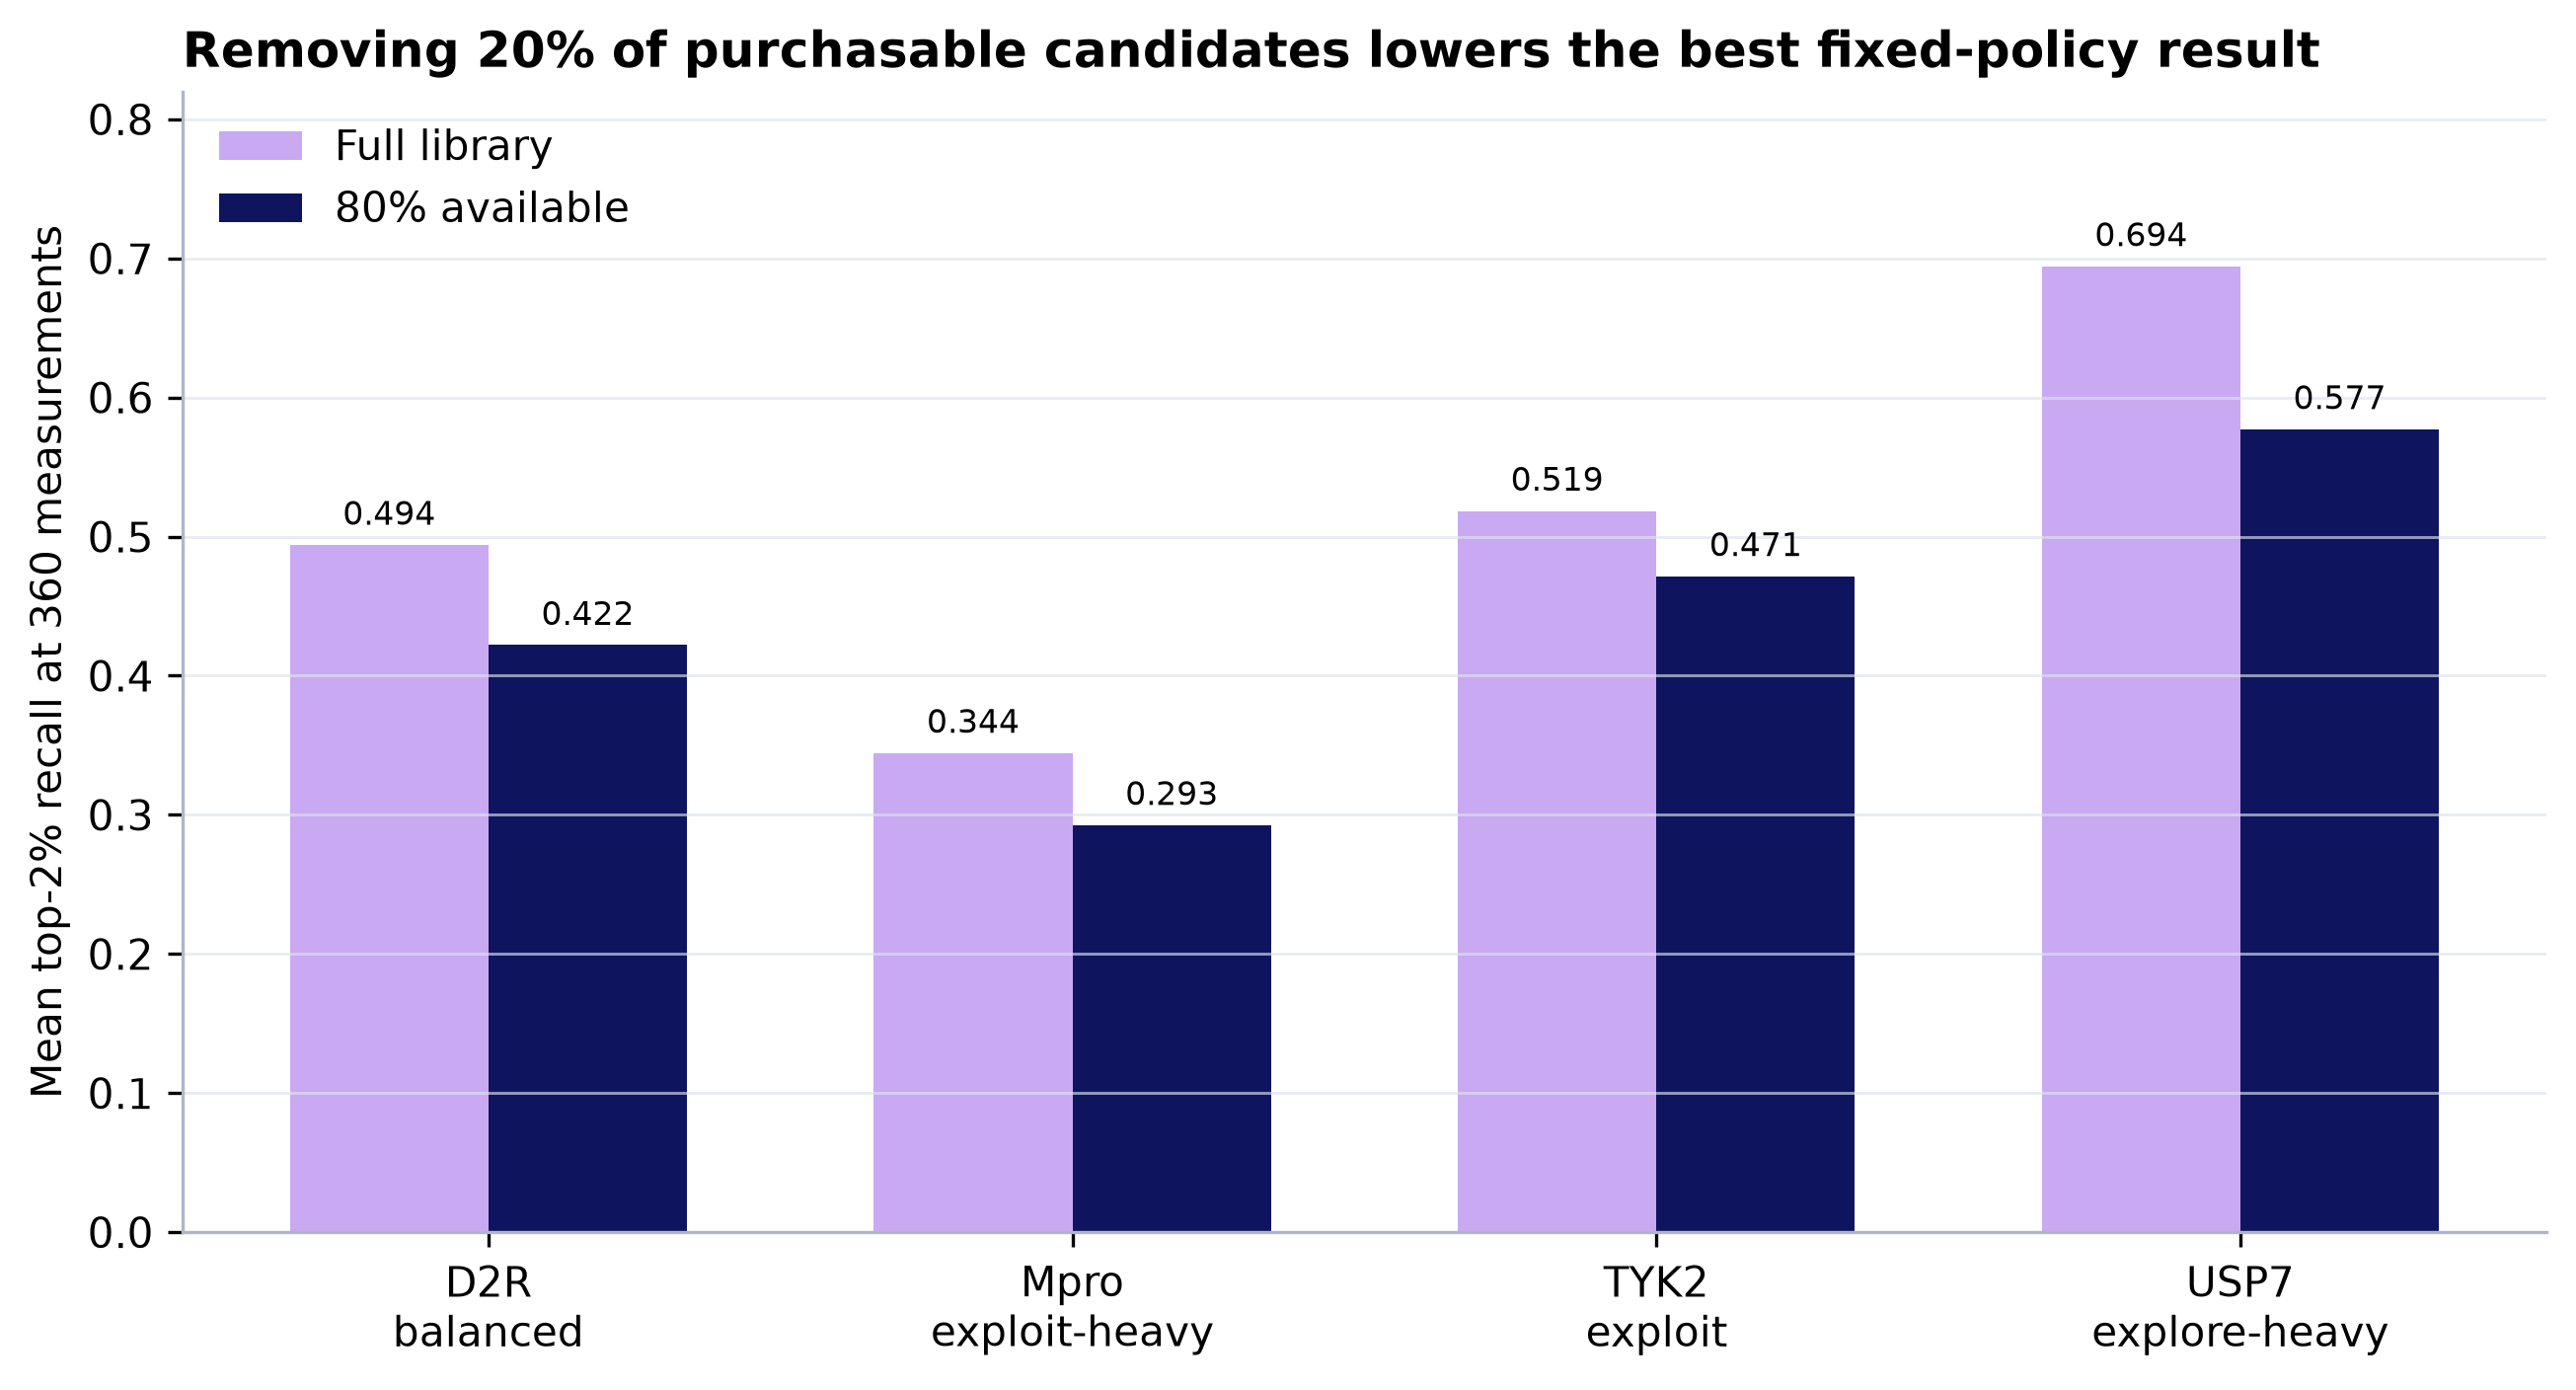
\includegraphics[width=\linewidth]{figures/availability_policy_comparison.png}
    \caption{Change in each target's strongest constrained fixed policy relative to the same unconstrained policy. Availability lowers attainable recall for every leader.}
\end{figure}

\section{Reproducibility and validation}

All seven Zenodo artifacts matched their published byte sizes and MD5 checksums, and the archive integrity check passed. The fixed benchmark contains 360 complete campaigns and 3,960 trajectory rows. The core agent benchmark contains 40 campaigns, 440 trajectory rows, and 400 decisions. The information-ablation benchmark contains 200 campaigns and 2,000 decisions. The constrained fixed and agent benchmarks contain 360 and 40 campaigns, respectively. Initial sets, cycle budgets, allocation totals, unique selections, and availability masks were validated. The expanded test suite passed 40 tests. Ten early D2R ablation-gate sessions omitted a redundant top-level digest field; reconstructed digests and paired initial sets matched, yielding a documented \texttt{PASS\_WITH\_WARNING} rather than a failed validation.

The optional paid API replication was not run because neither an API key nor the explicit paid-check flag was supplied. A fail-closed runner and frozen configuration are included in the codebase for a 20-decision D2R check if exact response identifiers, model snapshot, token accounting, and latency become necessary.

\section{NeurIPS paper checklist}

\begin{enumerate}[leftmargin=*]
    \item \textbf{Claims.} \answerYes{} The abstract, results, and conclusion distinguish improvement over random from comparison with the strongest fixed policy and state limitations.
    \item \textbf{Limitations.} \answerYes{} Limitations of retrospective labels, target count, fixed surrogate choices, forecast scoring, and non-snapshot inference are described.
    \item \textbf{Theory.} \answerNA{} The paper makes no new theoretical claim.
    \item \textbf{Reproducibility.} \answerYes{} Dataset provenance, frozen campaign settings, paired seeds, metrics, validation, and optional snapshot replication are documented.
    \item \textbf{Code and data.} \answerYes{} Code, configurations, decisions, trajectories, summaries, and source provenance are organized in the accompanying anonymized supplement; public links should be inserted only in a deanonymized version.
    \item \textbf{Experimental details.} \answerYes{} Initial size, batch size, cycles, representation, surrogate, kernel, targets, replicates, ablations, and availability construction are specified.
    \item \textbf{Statistical reporting.} \answerYes{} We report paired means, ten seeds, and percentile-bootstrap intervals; no unsupported significance claim is made where intervals cross zero.
    \item \textbf{Compute.} \answerTODO{} Wall-clock time and hardware totals should be added from execution logs before submission.
    \item \textbf{Human subjects.} \answerNA{} No human participants or annotators were used.
    \item \textbf{Personally identifiable information.} \answerNA{} The molecular datasets contain no personal data.
    \item \textbf{Licenses.} \answerTODO{} The final supplement should reproduce the upstream code and Zenodo artifact licenses verbatim.
    \item \textbf{Potential harms.} \answerYes{} The discussion notes prospective-validation and dual-use considerations for chemical discovery.
    \item \textbf{Use of agents and LLMs.} \answerYes{} The language model is the studied controller and is described in the experimental setup; it is not listed as an author.
\end{enumerate}

\end{document}
